\documentclass[12pt,twoside,a4paper]{report}
%\usepackage{ngerman}
\usepackage[ngerman,english]{babel}
%\usepackage[latin1]{inputenc}
\usepackage[reqno]{amsmath}
\usepackage{natbib}
\usepackage{anysize}
%\usepackage{sidecap}
%\marginsize{3.0}{1.0}{1.0}{1.0}

\usepackage{pslatex}
\usepackage{graphicx}
\usepackage{color}
\definecolor{Gray}{gray}{0.5}
\usepackage[margin=10pt,font=small,labelfont=bf]{caption}
\usepackage[position=top,singlelinecheck=false]{subfig}
\usepackage{multirow}
\usepackage{lscape}
\usepackage[verbose]{placeins}
%\usepackage{longtable}
\setlength{\parindent}{0mm}
\numberwithin{equation}{chapter}
\numberwithin{figure}{chapter}
\numberwithin{table}{chapter}
\usepackage{amssymb}

% Kopf- und Fusszeilen definieren
\usepackage{fancyhdr}
\pagestyle{fancy}
\renewcommand{\headrulewidth}{0.4pt}
\fancyhead[RO,LE]{\thepage}
\fancyhead[RE]{\slshape \rightmark}
\fancyhead[LO]{\slshape \leftmark}
\fancyfoot[C]{}

% Aendern der Schriftart
\usepackage{mathptmx}
\usepackage[scaled=0.92]{helvet}
%\renewcommand{\familydefault}{\sfdefault}
% Changing font for mathcal
\DeclareMathAlphabet{\mathcal}{OMS}{cmsy}{m}{n}

% adding hyperref package
% - adding backlinks in bibliography by option pagebackref
\usepackage[colorlinks, linkcolor = black, citecolor = black, filecolor = black, urlcolor = blue]{hyperref}

\usepackage{eso-pic}
\usepackage{color}

\usepackage{bibentry}
\nobibliography*
% define depth of table of content
\setcounter{tocdepth}{2}


%----------------------------------------------------------------------
% my definitions
\DeclareMathOperator\Sdd{\mathrm{d}}


\begin{document}

%-------------------- Titelseite --------------------%
\thispagestyle{empty}

\sffamily

\AddToShipoutPictureBG*{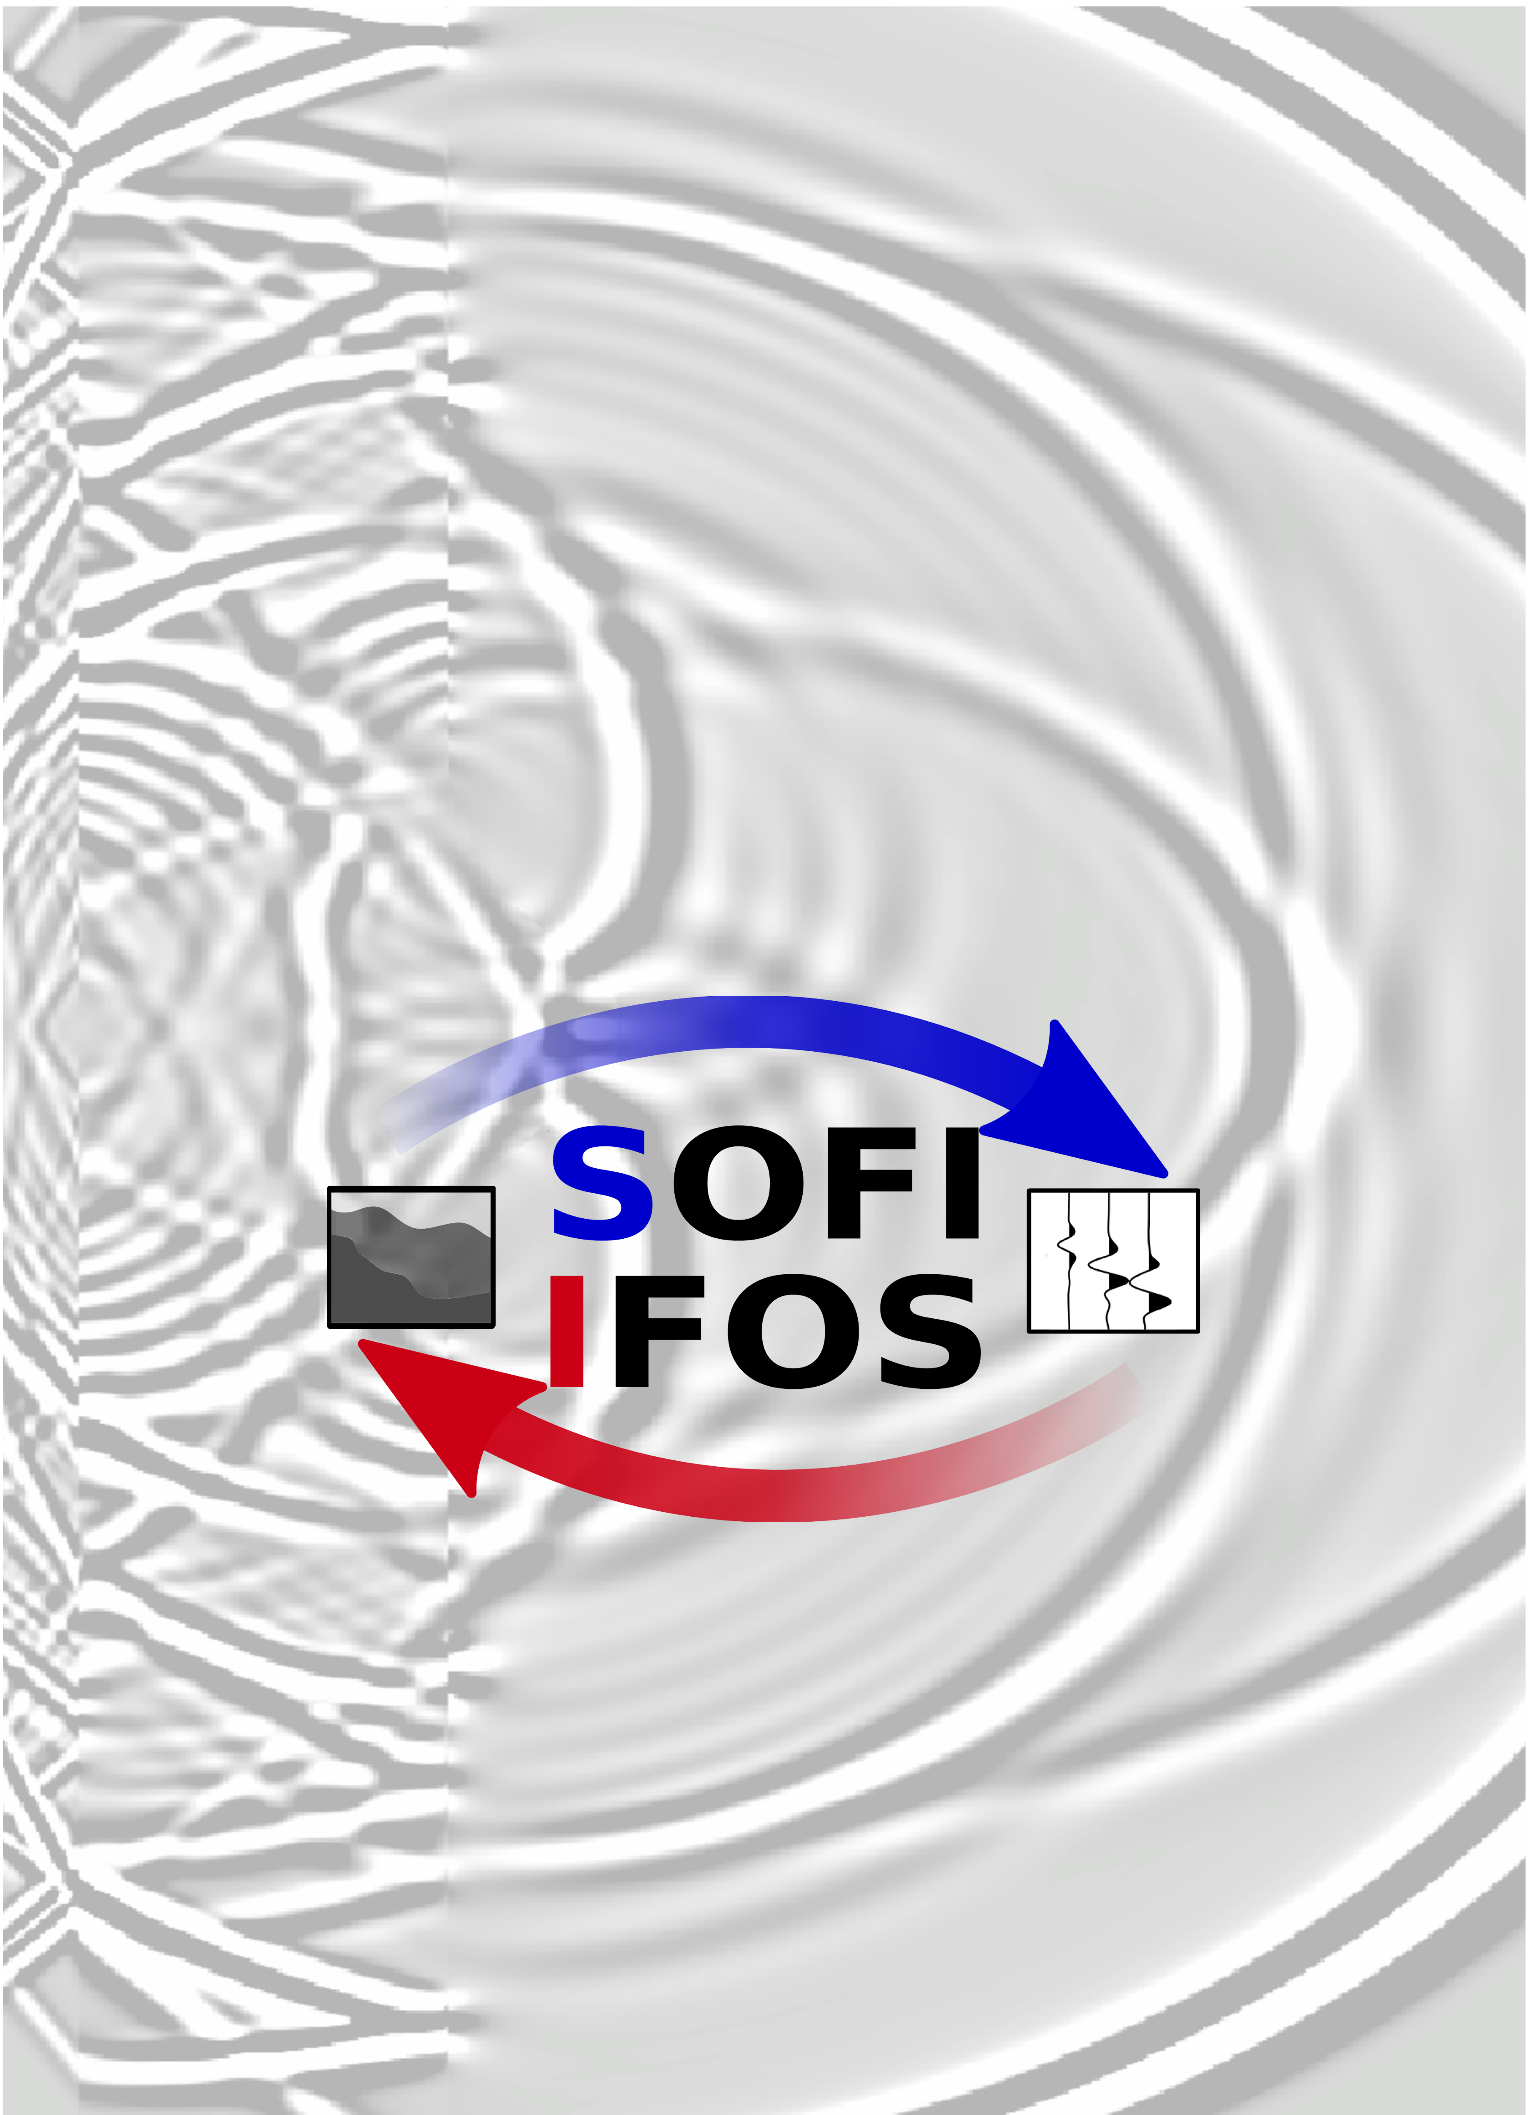
\includegraphics[width=\paperwidth,height=\paperheight]{fig/title_page1_sofi_ifos.pdf}}

\noindent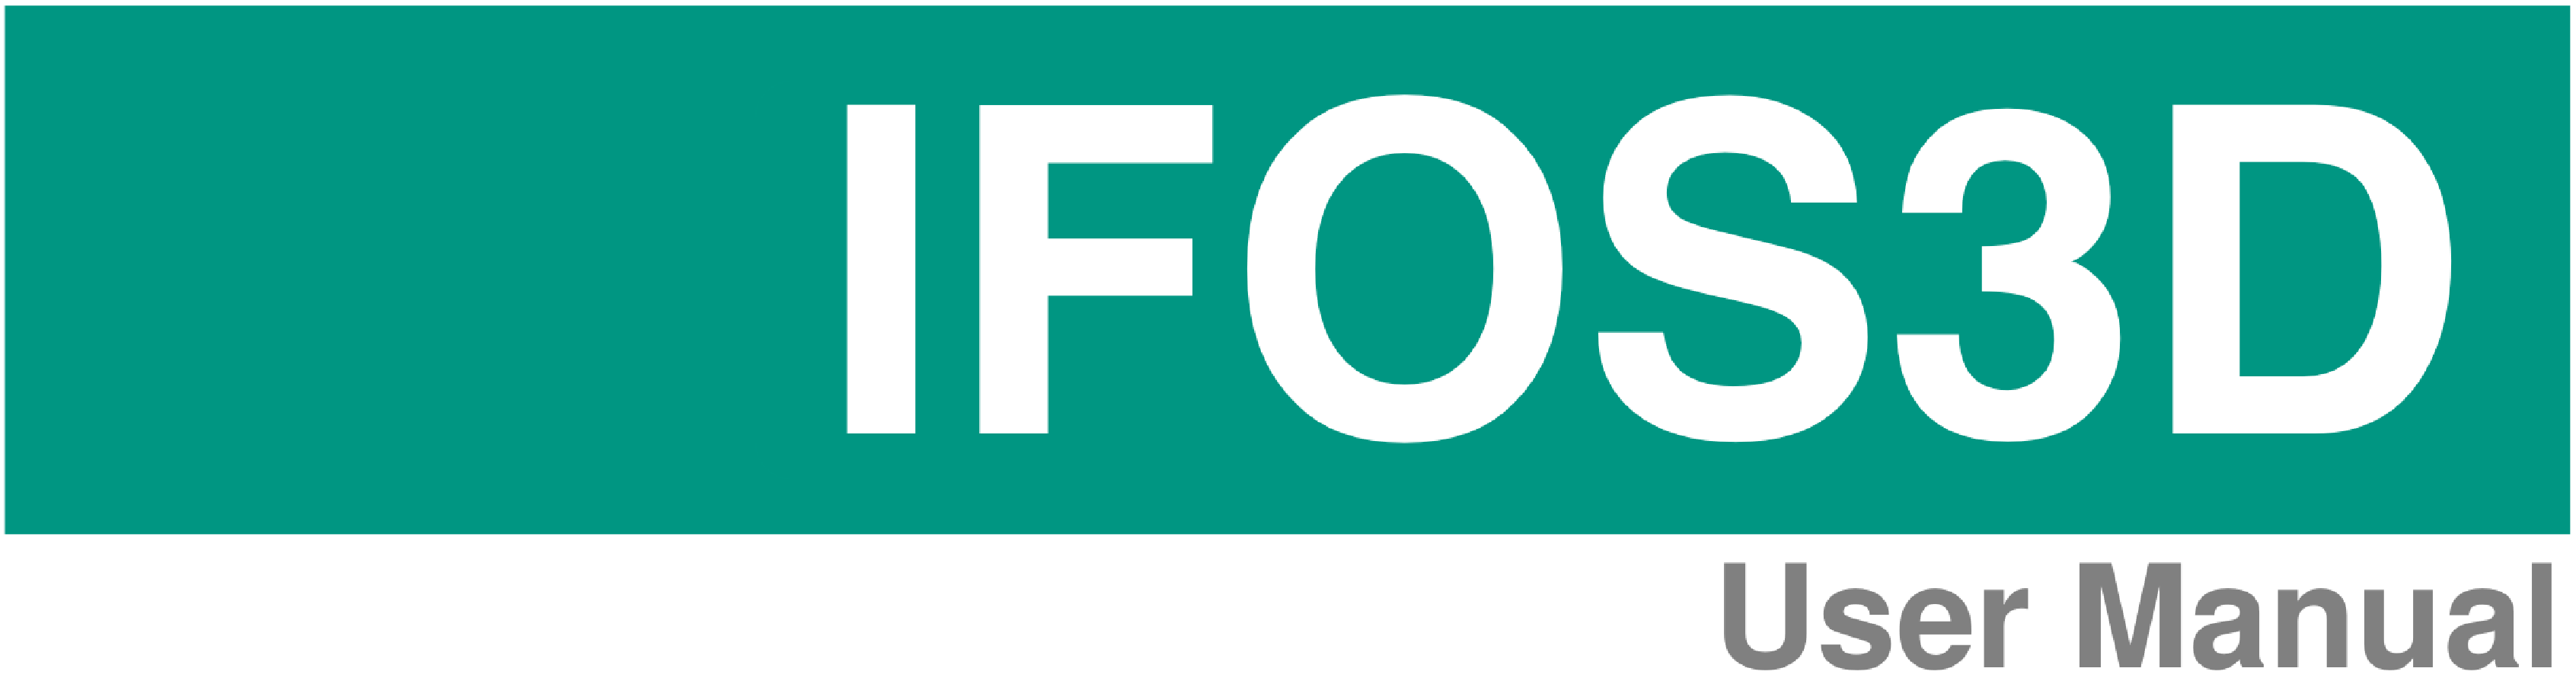
\includegraphics[width=1.0\textwidth]{fig/IFOS3D_title1.pdf}

\vspace{0.3 \textwidth}

%\begin{center}
%\includegraphics[width=.7\textwidth]{fig/logo_SOFI_IFOS.eps}

%\vspace{0.2\textwidth}

%\end{center}
\rmfamily

\FloatBarrier
\newpage 
\thispagestyle{empty}
\quad 
\newpage

\pagestyle{fancy}
%-------------------- Titelseite (Ende) --------------------%
%\input{Abstract.tex}
%\cleardoublepage


\pagenumbering{Roman}

\section*{Authors}

The IFOS3D code was first developed by Simone Butzer at the Karlsruhe Institute of Technology (KIT) from 2009-2014. Contributions were given by Andre Kurzmann and Lisa Groos.\\
\newline
The forward code is based on the viscoelastic FD code SOFI3D by \cite{boh02}.\\
\newline
Different external libraries for time domain filtering are used. The copyright of the source codes are held by different persons:\\
\newline
cseife.c, cseife.h:\\ 
Copyright $\copyright$ 2005 by Thomas Forbriger (BFO Schiltach) \\
\newline
cseife\_deriv.c, cseife\_gauss.c, cseife\_rekfl.c, cseife\_rfk.c and cseife\_tides.c:\\
Copyright $\copyright$ 1984 by Erhard Wielandt\\
This algorithm was part of seife.f. A current version of seife.f can be obtained from http://www.software-for-seismometry.de/\\
\newline 
The Matlab implementation of a few SU routines, mainly used to read and write SU files are:\\
Copyright $\copyright$ 2008, Signal Analysis and Imaging Group\\
For more information: http://www-geo.phys.ualberta.ca/saig/SeismicLab\\
Author: M.D.Sacchi\\
\newline

%\noindent
%Since then it has been developed and maintained by a development team: in alphabetical order,\\
%\newline
%(since 2015)\\
%...
% (add other developers here in the future).

\newpage

\section*{License}\label{license}

IFOS3D is free software: you can redistribute it and/or modify it under the terms of the GNU General Public License as published by the Free Software Foundation, version 2.0 of the License only.\\
 \newline
IFOS3D is distributed in the hope that it will be useful, but WITHOUT ANY WARRANTY; without even the implied warranty of MERCHANTABILITY or FITNESS FOR A PARTICULAR PURPOSE. See the GNU General Public License for more details. You should have received a copy of the GNU General Public License along with IFOS3D. See file COPYING and/or \path{http://www.gnu.org/licenses/gpl-2.0.html}.\\
\newline
The Authors of IFOS3D are listed in file \path{AUTHORS}.
%------------------------------------------------------------------------------------------------%
\section*{Acknowledgments}
%------------------------------------------------------------------------------------------------%

We thank the seismic working group of the Geophysical Institute at KIT for constructive discussions. 

\noindent The development of the code was supported by the Karlsruhe Institute of Technology (KIT), the Deutsche Forschungsgemeinschaft (DFG), the Bundesministerium f\"ur Bildung und Forschung (BMBF) and the Wave Inversion Technology (WIT) Consortium.

\noindent The code was tested and optimized at the computing centres of the Karlsruhe Institute of Technology (KIT), the supercomputing center in Juelich and the HLRS in Stuttgart. 
\newline

%------------------------------------------------------------------------------------------------%
\section*{References}
%------------------------------------------------------------------------------------------------%

\noindent\bibentry{But13}\\

\noindent\bibentry{But15}\\

\tableofcontents
\cleardoublepage
\pagenumbering{arabic}

%Implementation FWI
\chapter{Introduction}
In the 1980's \cite{Lai83}, \cite{Tar84} and \cite{Mor87} suggested a new inversion strategy known as full waveform inversion (FWI). This method aims to reconstruct multi-parameter images of the subsurface by iteratively minimising the misfit between modeled and observed data. Thus it takes the full information content of the seismograms into account and can offer a significantly improved resolution compared to conventional methods. The optimisation problem is generally solved with gradient-based methods, which can be implemented very efficiently for FWI using the adjoint approach \citep[e.g.][]{Tar84, Mor87}. \\
Different approximations are generally used to limit the large number of unknown subsurface parameters and to mitigate the computational costs of the inversion. Many applications are performed in the 2D approximation. This leads to an enormous decrease of the number of subsurface parameters. Still, the 2D approximation is unable to explain 3D scattering and can lead to artefacts in 3D heterogeneous medium. Furthermore the use of a 3D FWI offers the possibility to invert for 3D structures and to gain a 3D image of the subsurface. Often, wave propagation in FWI applications is described with the (visco-) acoustic wave equation. Herby only compressional waves are considered which can be sufficient in marine seismics. However, in land seismics the abundance of shear waves and surface waves favours the (visco-) elastic wave equation. Still,  studies on the implementation and application of 3D elastic FWI as performed by \cite{Epa08}, \cite{Fic09},  \cite{Cas11}, \cite{Gua12} and \cite{But13} are rare and computationally expensive.\\
\\
IFOS3D is a 3D elastic full waveform inversion tool which aims to resolve the elastic parameters (compressional and shear wave velocity and density) of the 3D subsurface. It is based on the conjugate gradient method. For a good computational performance the gradient is calculated with a time-frequency approach. Hereby the wavefields are simulated with the fast and efficient finite-difference forward solver SOFI3D in time domain \citep{boh02}. The gradient calculation is then performed in frequency domain for discrete frequencies. A discrete Fourier transform on the fly enables the transformation from time to frequency domain. For an optimisation of the gradient method IFOS3D offers the calculation of a diagonal Hessian approximation and application of the L-BFGS method.\\
The IFOS3D program is an extension of the SOFI3D forward modeling code for inversion and is thus closely linked to this program. SOFI3D is based on the FD approach described by \cite{Vir86} and \cite{Lev88}. The present program SOFI3D (elastic version) has the following extensions
\begin{itemize}
\item employs higher order FD operators,
\item applies Perfectly Matched Layer boundary conditions at the edges of the numerical mesh \citep{Kom07},
\item works in MPI parallel environment ONLY, i.e. SOFI3D is a implementation based on a domain decomposition
\citep{boh02}.
\end{itemize}
The manual of SOFI3D gives a detailed description of the forward modelling solver, its features and the corresponding input parameters.\\
\\
IFOS3D was successfully tested in different synthetic applications including transmission and surface acquisition geometries \citep{But13,But15}. A detailed description of the theory and implementation of the program is given by \cite{But15}. This manual will give an overview about the structure and implementation of IFOS3D which is necessary to run the program. The different input parameters are decribed in detail. Additionally IFOS3D comes with a toy example which is described in this guide. It can be performed in a few steps and therefore offers a good access to IFOS3D.
 
\clearpage
\chapter{Theory and implementation}
\section{The inverse problem}
Full waveform inversion (FWI) aims to minimise the misfit between modeled and observed data to find a subsurface model $\textbf m$ which explains the observed data optimally. IFOS3D uses the $L_2$-norm based misfit function $E$ given by 
\begin{equation}E(\textbf m)=\frac{1}{2}\sum_{s}\int_0^T dt \sum_{r}\delta u_i(\textbf x_s,\textbf x_r,t)^2, \label{eq:L2}\end{equation}
with the $i$-th component of the displacement residual $\delta u_i=u_i-u_{i,obs}$ at source position $\textbf x_s$ and receiver position $\textbf x_r$. $\textbf u_{obs}$ denotes the observed data, whereas $\textbf u$ denotes the modelled data. The squared residuals are summed up over all sources $s$ and receivers $r$ and integrated over time $t$ for the full record length $T$. In this and the following equations we use the Einstein notation to sum up over double indices.
\subsection*{The gradient methods}
A conjugate gradient approach is applied to solve this optimisation problem. Gradient methods are local inversion methods, which iteratively minimise the misfit by updating the model in the direction of the steepest descent of $E$. The model in iteration $k$ is updated by 
\begin{equation} \textbf m_{k+1}=\textbf m_k-\alpha_k\textbf p_k \hspace{0.4cm}\text{with} \hspace{0.4cm}\textbf p_k=\textbf P\nabla_mE_k. \label{equ:update1} \end{equation}
Hereby $\nabla_mE_k$ is the gradient of the misfit function, $\textbf P$ is a preconditioning operator, which mitigates amplitude effects in the gradient, and $\alpha_k$ is the step length. Gradient directions in FWI can be implemented very efficiently with the adjoint approach \citep[e.g.][]{Tar84, Mor87} and these methods are thus applicable even for larger problem sizes. Note however, that the misfit function in FWI is generally very rough and contains local minima. In order to reach the global minimum with this local inversion method, a good starting model and the application of inversion strategies, like frequency filtering are essential. \\
The use of the conjugate gradient $\textbf c_k$ compared to the general gradient $\nabla_mE_k$ can improve the convergence. The conjugate gradient direction $\textbf c_k$ in iteration $k$ is given by 
\begin{equation}\textbf c_k=\textbf P\nabla_m E_k+\beta_k\textbf c_{k-1}. \label{equ:conjgrad1} \end{equation} This stabilises the inversion by adding some part of the previous gradient.  The scalar $\beta$ is estimated with the Polak-Ribi\'{e}re method as 
\begin{equation}\beta_k=\frac{\textbf p_k^T(\textbf p_k-\textbf p_{k-1})}{||p_{k-1}||^2}\hspace{0.15cm} \text{for} \hspace{0.15cm}\beta_k>0; \hspace{0.5cm}\beta_k=0 \hspace{0.15cm}\text{for} \hspace{0.15cm}\beta_k<0.\label{equ:beta}\end{equation}
The distinction of cases ensures, that the model is updated in the decent direction of the misfit function. The new model is then estimated as
\begin{equation}\textbf m_{k+1}=\textbf m_k-\alpha_k\textbf c_k. \label{equ:conjgrad2} \end{equation}

\section{Forward modeling with SOFI3D}
Before explaining the inversion process, we will shortly describe the solution of the forward problem. 3D  elastic FWI requires a forward solver, which accurately simulates seismic wave propagation in the elastic media. Otherwise artefacts and deviations in the inversion result can be caused by fitting modelling errors in the wavefield. Additionally, a computationally efficient forward solver is required, because the inversion process is characterised by a high number of forward modellings and the FWI runtime is thus mainly influenced by the runtime spend for wavefield modelling. \\
``IFOS3D'' uses the elastic version of the time-domain finite-difference solver ``SOFI3D'' \citep{boh02} for wavefield modelling, which very efficiently and fast solves the 3D elastic wave equation. The code discretizes the velocity stress formulation of the elastic wave equation on a staggered grid \citep{Vir86, Lev88}. It is able to accurately model wave propagation in 3D complex media. A viscoelastic version of SOFI3D exits, but was not tested for FWI yet. In the following, I will give a short overview of SOFI3D and its characteristics, but refer to the SOFI3D manual for a more detailed description of its theory, implementation and performance.\\
Wave propagation can be described in the velocity-stress formulation. This formulation uses the particle velocity $\textbf v=\partial\textbf u/\partial t$ as wavefield parameter. For the elastic isotropic medium wave propagation due to a force $\textbf f$ can then be described as first order differential equations:
\begin{equation}
 \begin{split}
  \rho\frac{\partial v_i}{\partial t}=f_i+\frac{\partial\tau_{ij}}{\partial x_j},\\
\frac{\partial\tau_{ij}}{\partial t}-\lambda\frac{\partial\Theta}{\partial t}\delta_{ij}+2\mu\frac{\partial\epsilon_{ij}}{\partial t}=0,\\
\frac{\partial\epsilon_{ij}}{\partial t}=\frac{1}{2}\left (\frac{\partial v_i}{\partial x_j}+\frac{\partial v_j}{\partial x_i}\right ).
 \end{split}\label{equ:wave_equvel}
\end{equation}
The elastic medium is described by the density $\rho$ and the Lam\'e parameters $\lambda$ and $\mu$. $\tau_{ij}$ denotes the elements of the stress tensor and $\epsilon_{ij}$ denotes the elements of the strain tensor. The trace of the stress tensor is given by $\Theta$.
\subsection{Finite difference modeling}\label{sec:FDmodeling}
For the simulations of 3D elastic wave propagation these equations are approximated by finite differences (FD). For the calculation of partial derivatives, the wavefield parameters and model parameters are discretised on a staggered-grid system \citep{Vir86, Lev88}. The 3D staggered-grid system is sketched in Figure~\ref{fig:stag_grid}. We use a Cartesian grid (x,y,z)=(i,j,k). The model parameters $\lambda$, $\mu$ and $\rho$ and the diagonal stress components $\sigma_{ii}$ are localised on the full grid points, whereas velocities and off-diagonal stress components are calculated on a grid which is half a grid point shifted to the original system. Compared to a conventional Cartesian grid, the staggered grid enables a larger grid spacing for the same level of accuracy.\\
\begin{figure}
\centering
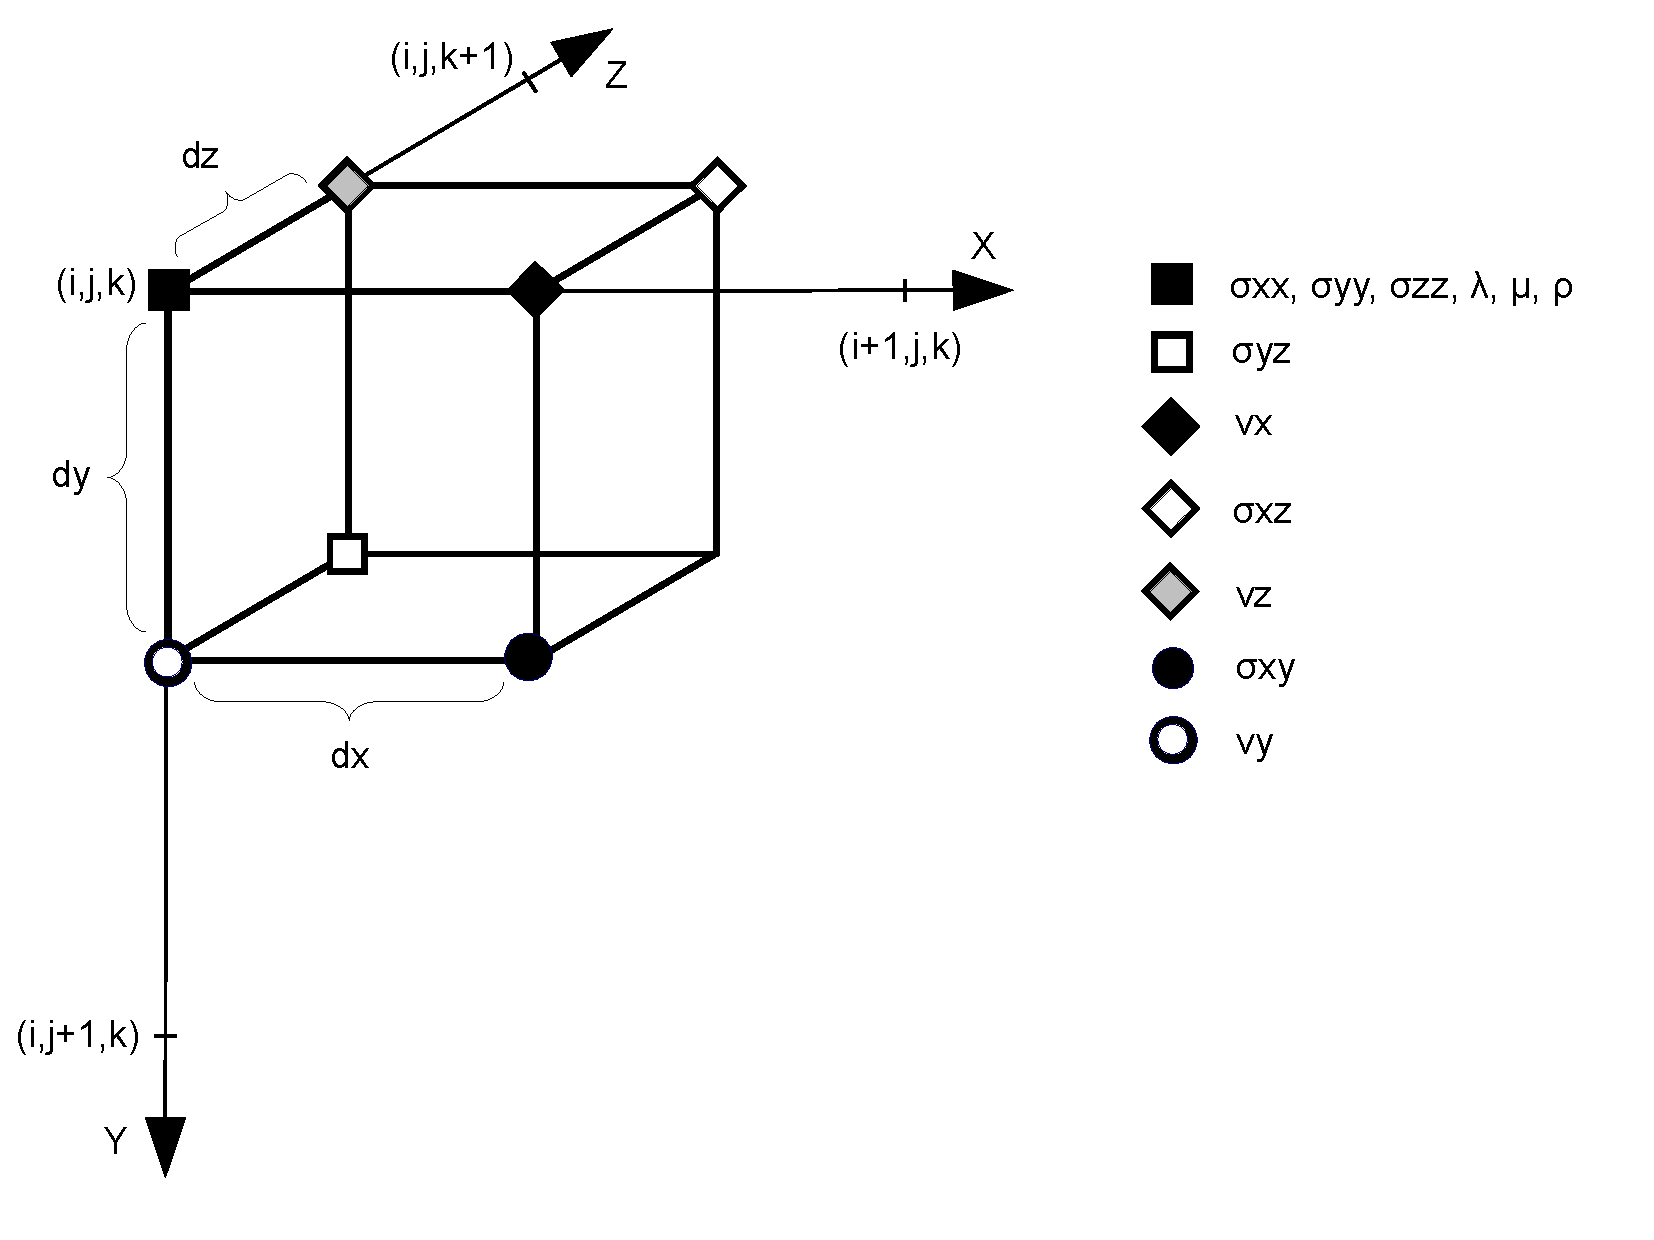
\includegraphics[width=0.74\textwidth]{fig/ssg_grid}
\caption[Staggered grid system]{Staggered-grid coordinate system used for 3D FD modelling in SOFI3D}\label{fig:stag_grid}
\end{figure}
The derivatives are approximated by centered finite differences. The easiest finite-differences are of second order, where the two adjacent grid points with a grid space $dh$ are used to calculate the derivative between these grid points as follows
\begin{equation}
 \frac{\partial f(x)}{\partial x}|_{i+1/2}\approx \frac{f[i+1]-f[i]}{dh}
\end{equation}
 The consideration of additional grid points in higher order schemes can increase the accuracy and thus enable a larger grid spacing. However, it needs to be considered, that the number of operations increases and the number of parameters which are interchanged during MPI communication rises. Additionally, high order finite-difference operators can cause problems in case of large discontinuities, like tunnels. The SOFI code uses second order temporal and second to 12th order spatial finite difference operators, which can be chosen according to the problem.\\
To solve the system of equations~\ref{equ:wave_equvel} two steps are performed for each time step: 
\begin{itemize}
 \item velocity updates are calculated using spatial stress derivatives and are added to the previous velocity values
\item stress value updates are calculated using spatial velocity derivatives and Hook's law and are summed to the previous stress values
\end{itemize}
Hereby the summation of the update values over all time steps accounts for the time derivatives of velocity and stress values. 
\subsection{Additional charactersistics of SOFI3D}\label{sec:SOFI3Dcharacter}
\subsubsection*{Boundary conditions}
There are two ways to avoid arteficial reflections from model boundaries in SOFI3D. The first exponentially damps waves within a boundary zone surrounding the model by multiplying the amplitudes with an exponentially decaying factor \citep{Cer85}. At least 30 gridpoints thickness at boundary zones is required. The second method is the implementation of convolutional perfectly matched layers (C-PMLs) \citep{Ber94,Kom07}. This method can offer a much better performance compared to the  conventional exponential damping and a boundary zone of 10 gridpoints thickness is generally sufficient. However, in case of strong contrasts and heterogeneities at the model boundary instabilities can be caused.
\subsubsection*{The free surface}
At the free surface, the vertical stress components $\sigma_{xy}$, $\sigma_{yy}$ and  $\sigma_{zy}$ are zero. A planar free surface is implemented implicitely in SOFI3D with the mirroring technique described by \cite{Lev88}.
\subsubsection*{Grid dispersion and stability} 
To mitigate numerical dispersion and grid anisotropy of the wavefield the grid spacing must be chosen sufficiently small. For a fourth-order spatial and second-order temporal scheme the criterion 
\begin{equation}
 dh < \frac{\lambda_{min}}{6}=\frac{v_{min}}{6f_{max}} \label{equ:grid_disp}
\end{equation}
ensures a wavefield error of less than 5\% \citep{boh02}. It depends on the minimum wavelength $\lambda_{min}$, defined by the minimum velocity $v_{min}$ and the maximum frequency $f_{max}$.  Higher order FD-operators enable a larger grid spacing.\\
In order to ensure stability of the simulation, the temporal spacing must satisfy the Courant-Friedrichs-Levy (CFL) stability criterion \citep{Cou67}. It is related to the maximum velocity $v_{max}$ and is given by
\begin{equation}
 dt<=\frac{dh}{h\sqrt{3}v_{max}}.
\end{equation}
The constant factor $h$ amounts to $\frac{7}{6}$ for a Taylor operator of fourth order. For different FD orders and Holberg coefficients we refer to the SOFI manual.
\subsubsection*{Viscoelasticity}
A viscoelastic version of SOFI3D exists. For its implementation we refer to \cite{boh02}. So far we only employed the elastic version of SOFI3D for IFOS3D. However, it would be possible to include the viscoelastic update functions. This enables the use of viscoelasticity as passive parameter in the inversion process. This could already be successfully tested for the 2D elastic FWI with IFOS2D.	
\section{The inversion process - overview}
Figure \ref{fig:workflow} explains the different steps, which are performed within each iteration of the conjugate gradient algorithm in IFOS3D. Each iteration can be divided into three parts. First, the misfit gradient $\Delta E_k(\textbf m)$ for each shot and model parameter ($\textbf m$) is calculated. Second, to calculate the search direction ($\textbf{c}_k$), the misfit is summed up over all shots, preconditioned and the conjugate gradient $\textbf c_k$ is calculated. Third, a step length estimation is performed, which determines the total size of the update. IFOS3D additionally enables the calculation of a diagonal Hessian approximation and the use of the L-BFGS sheme, which will be described in section \ref{sec:hess} and \ref{sec:lbfgs}, respectively.\\
The conjugate gradient method is realised with a time-frequency approach \citep{Sir08}. Wavefield modeling is performed in time domain using the finite difference solver SOFI, whereas the gradient is calculated in frequency domain. A discrete Fourier transformation on the fly is applied to calculate the frequency domain wavefields. The main advantage of the frequency domain inversion is the possibility to calculate the gradient only for few discrete frequencies \citep[e.g.][]{Pra99,Sir04,Bro09}. This results in an enormous reduction of storage costs compared to a time domain inversion, which generally requires the storage of the full forward field. The time-frequency approach additionally allows the use of the efficient and fast 3D time-domain FD forward solver. Thus, for 3D elastic FWI it is recommendable regarding computational performance. 
\begin{figure}[h!]
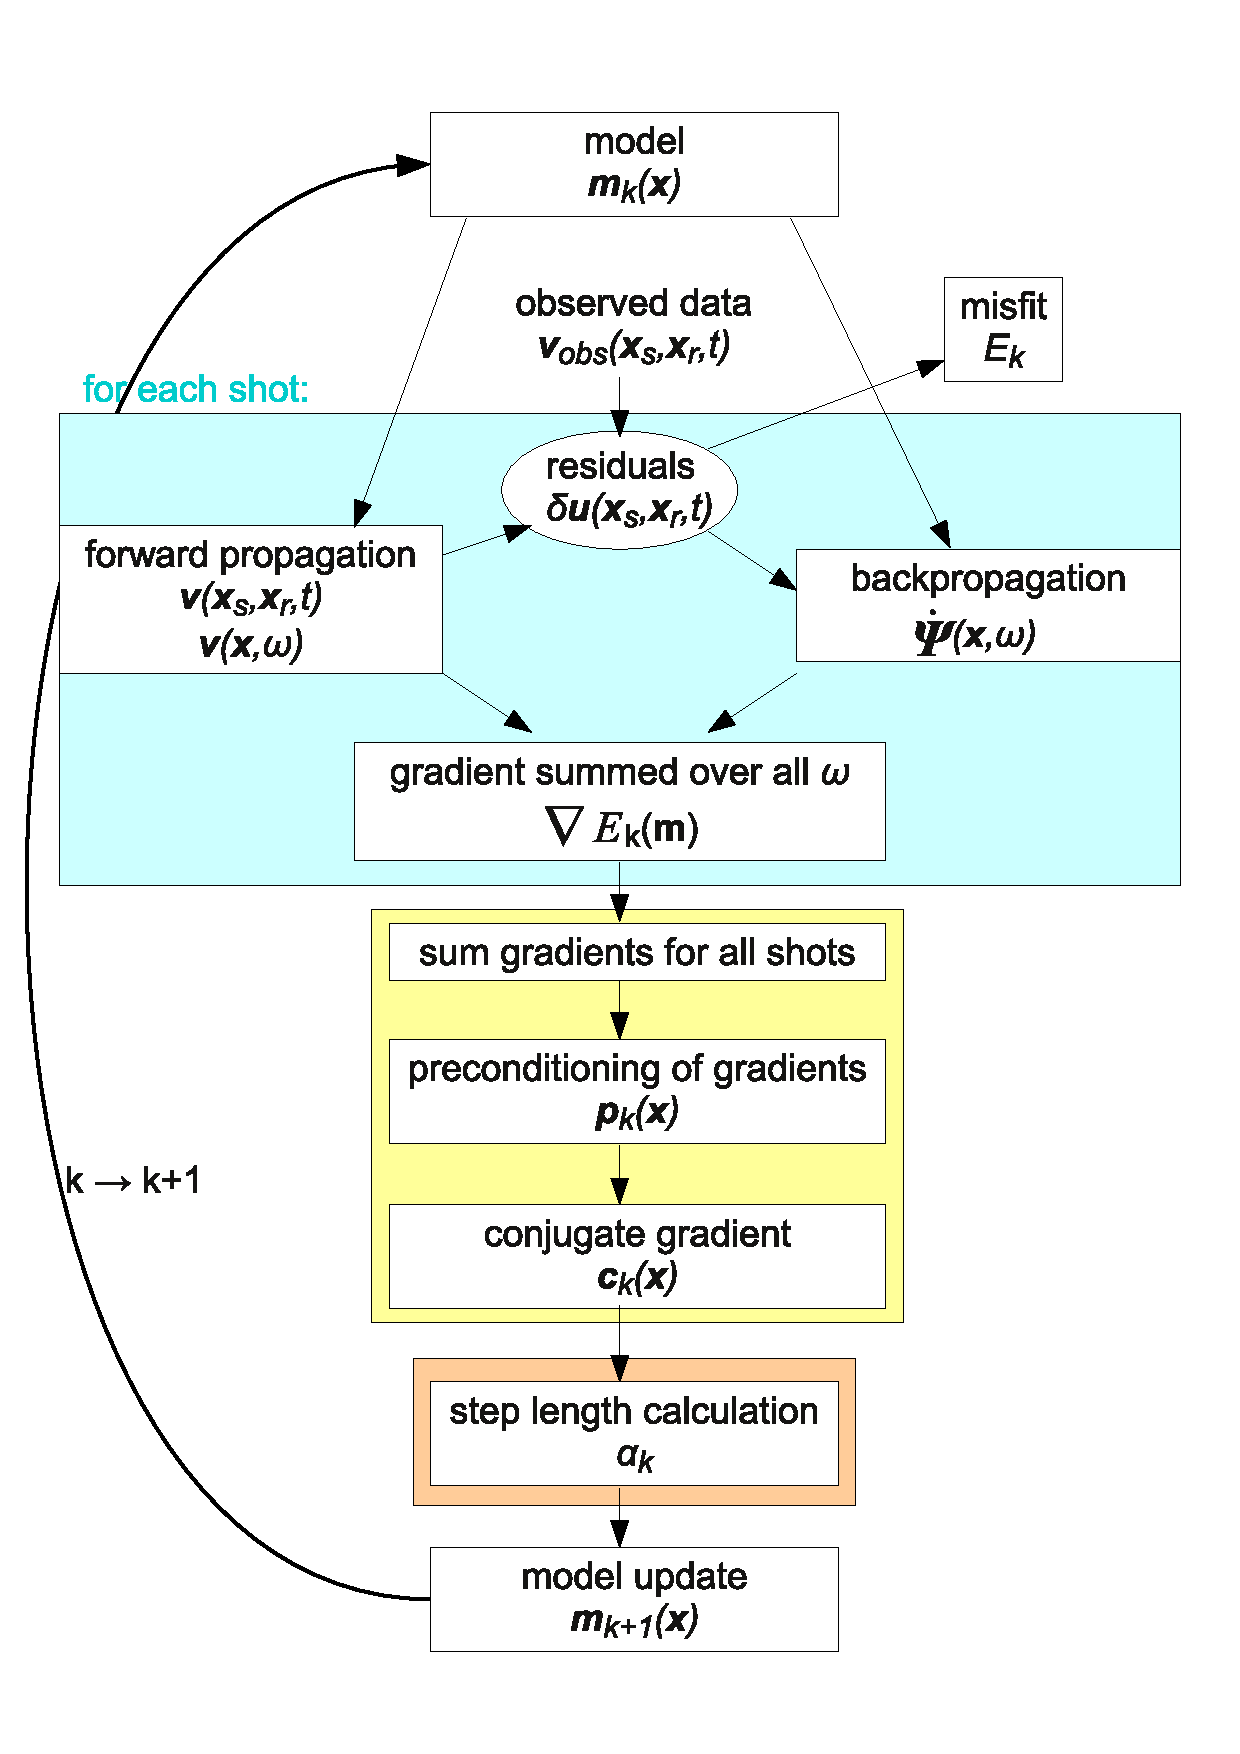
\includegraphics[width=0.9\textwidth]{fig/workflow}
\caption[IFOS3D workflow]{The workflow of IFOS3D shows the different steps performed during each iteration.}\label{fig:workflow}
\end{figure}

\section{Gradient calculation}\label{sec:grad_calc}
The misfit gradient is calculated with the adjoint method, which can be derived from perturbation theory \citep[e.g.][]{Tar84, Mor87}. The blue box of the workflow in Figure~\ref{fig:workflow} gives a sketch of its implementation and shows the gradient as multiplication of the forward wavefield and the conjugate adjoint wavefield. A detailed derivation of the gradient equations in IFOS3D is given by \cite{But15}. Here, we will only give a short overview about the employed equations and concentrate on the implementation.
\subsection{Extraction of monochromatic wavefields}
For the gradient calculation in frequency domain wavefield parameters of the forward and backpropagated wavefields are required for discrete frequencies. We follow the approach by \cite{Sir08} and use the discrete Fourier transformation
\begin{equation}\tilde{A}_i(\textbf x,\omega)=\sum_{l=0}^{nt}\exp(i\omega l\Delta t)A_i(\textbf x,l\Delta t)\Delta t, \label{equ:discFourier}  \end{equation}
 to extract the monochromatic wavefields, where $nt$ is the number of timesteps, $\Delta t$ the time sampling and $A_i$ a wavefield parameter. The discrete Fourier transformation is performed on the fly, summing up Fourier summands of $A_i$ in each time step. Therefore, no storage of the time domain wavefields at different time steps is required. Furthermore, the number of additional operations is low, as long as the transformation is only performed for few frequencies. Thus, the change from time to frequency domain can be achieved at low extra costs.
\subsection{Wavefield calculation}
In a first step, the forward-propagated wavefield for the model $\textbf m_k$ is simulated, which travels from source into medium. At each receiver position the seismograms $v(\textbf x_r,t)$ are stored. Additionally, by applying a discrete Fourier transformation (equation~\ref{equ:discFourier}), we calculate the particle velocities $\tilde v(\textbf x,\omega$), which are stored in memory for each discrete inversion frequency and at each grid point.\\
At each receiver position the time-reversed, residual displacement seismograms  $\delta u_i(\textbf x_r,T-t')$ are estimated. This residual is back-propagated from all receivers into the medium simultaneously. The corresponding backpropagated wavefield is defined as \begin{equation} \Psi_j(\textbf x,T-\tau)=\sum_{r}\int_0^T dt' G_{ji}(\textbf x,\tau;\textbf x_r,t')\delta u_i(\textbf x_r,T-t').\label{equ:psi}\end{equation} 
Hereby we use the same forward solver, which is based on the first-order wave-equation and therefore calculates the time derivative $\partial\Psi/\partial t=\dot\Psi$. For the backpropagation, the time line is reversed and we calculate wavefields starting from time $T$ backwards. Same as for the forward propagation, we extract the frequency wavefields $\tilde{\dot\Psi}(\textbf x,\omega)$ on the fly. These frequency wavefields are stored in memory for each frequency.
\subsection{Gradient equations in time and frequency domain}
Finally the gradients are calculated as multiplication of the forward and conjugate adjoint wavefields for each frequency and summed up over all frequencies. In the following the corresponding equations are described in more detail.\\
In time domain the misfit gradients for the elastic parameters $\lambda$, $\mu$ and $\rho$ can be estimated as zero-lag cross-correlation between forward and backpropagated wavefields as \citep[e.g.][]{Mor87,But15}
\begin{equation}
\begin{split}
 \frac{\partial E(\textbf m)}{\partial\rho(\textbf x)} & =-\sum_{s}\int_0^T d\tau \frac{\partial\Psi_j(\textbf x,\tau)}{\partial\tau}\frac{\partial u_j(\textbf x,\tau)}{\partial\tau}
\\
\frac{\partial E(\textbf m)}{\partial\lambda(\textbf x)} & =-\sum_{s}\int_0^T d\tau \frac{\partial\Psi_j(\textbf x,\tau)}{\partial x_j}\frac{\partial u_p(\textbf x,\tau)}{\partial x_p}
\\
 \frac{\partial E(\textbf m)}{\partial\mu(\textbf x)} & =-\frac{1}{2}\sum_{s}\int_0^T d\tau \left (\frac{\partial\Psi_j(\textbf x,\tau)}{\partial x_k}+\frac{\partial\Psi_k(\textbf x,\tau)}{\partial x_j}\right )\left (\frac{\partial u_j(\textbf x,\tau)}{\partial x_k}+\frac{\partial u_k(\textbf x,\tau)}{\partial x_j}\right ).
\end{split}\label{equ:grad3}
\end{equation}
These equations can be transformed to frequency domain. Using Fourier transforms the wavefield in time domain $\textbf u(\textbf x,t)$ are transformed into frequency domain  $\tilde{\textbf u}(\textbf x,\omega)$ and backwards with
\begin{equation}
 \tilde{\textbf u}(\textbf x,\omega)=\frac{1}{\sqrt{2\pi}}\int_{-\infty}^{+\infty} \textbf u(\textbf x,t)e^{-i\omega t} dt  \hspace{0.8cm}  
 \textbf u(\textbf x,t)= \frac{1}{\sqrt{2\pi}}\int_{-\infty}^{+\infty}\tilde{\textbf u}(\textbf x,\omega)  e^{i\omega t} d\omega  \label{equ:fourier1}   \end{equation}
Additionally we use that the zero-lag cross-correlation of two real signals $A$ and $B$ in time domain is replaced by a multiplication of one signal with the conjugate of the other signal integrated over the full frequency spectra in frequency domain.
\begin{equation}
\int_{-\infty}^{+\infty}dtA(t)B(t) =\int_{-\infty}^{+\infty}d\omega \tilde{A}(\omega)\tilde{B}^*(\omega) \label{equ:fourier2}
\end{equation}
This is now applied to the time-domain gradient expressions in \ref{equ:grad3}. The time integration $\int_0^T d\tau$ can be extended to $\int_{-\infty}^{+\infty} d\tau$ if the condition of $\textbf u(\textbf x,t)=0$ and $\partial\textbf u(\textbf x,t)/\partial t=0$ for $t<0$ and $t>T$ is fulfilled. In the density gradient, the time derivatives each transform to frequency domain by multiplication with a factor of $i\omega$. Spatial derivatives are not affected by the transformation.\\
The gradients in frequency domain can then be expressed as 
\begin{equation}
\begin{split}
 \frac{\partial E(\textbf m)}{\partial\rho(\textbf x)} & =\sum_{s}\sum_{v=1}^{n_f}\textit{Re}[\omega_v^2 \tilde{u}_i(\textbf{x},\omega_v)\tilde{\Psi}_i^*(\textbf{x},\textbf x_s,\omega_v)]
\\
\frac{\partial E(\textbf m)}{\partial\lambda(\textbf x)} & =-\sum_{s}\sum_{v=1}^{n_f}\textit{Re}\left [\frac{\partial u_p(\textbf x,\omega_v)}{\partial x_p}\frac{\partial\Psi_j^*(\textbf x,\omega_v)}{\partial x_j}\right ]
\\
 \frac{\partial E(\textbf m)}{\partial\mu(\textbf x)} & =-\frac{1}{2}\sum_{s}\sum_{v=1}^{n_f} \textit{Re}\left [\left (\frac{\partial u_j(\textbf x,\omega_v)}{\partial x_k}+\frac{\partial u_k(\textbf x,\omega_v)}{\partial x_j}\right )\left (\frac{\partial\Psi^*_j(\textbf x,\omega_v)}{\partial x_k}+\frac{\partial\Psi^*_k(\textbf x,\omega_v)}{\partial x_j}\right )\right ].
\end{split}\label{equ:grad5}
\end{equation}
Hereby we replace the integral over the full frequency spectra by a summation over few discrete frequencies. The use of only few frequencies in contrast to the full spectra is possible in FWI as shown for example by \citep[e.g.][]{Sir04,Ple09,Bro11} as long as the wavenumber spectra is covered continously during inversion. However note that the better redundancy in time-domain FWI can lead to a better performance in case of complex wavefields \citep{Vir09}.
\subsection{Implementation of gradient calculation}
For each shot the  gradients are calculated using the stored forward wavefield $\tilde{v}(\textbf x,\omega$) and back-propagated wavefield $\tilde{\dot\Psi}(\textbf x,\omega)$ according to the equations~\ref{equ:grad5}. Hereby the gradient of $\rho$ can be calculated directly as multiplication of velocity components $\tilde{v}_i$ and $\tilde{\dot\Psi}_i$. To derive displacements $\tilde{u}_i$ and $\tilde{\Psi}_i$ as required for the computation of the gradients of $\lambda$ and $\mu$, the frequency domain enables a simple integration with 
\begin{equation}\tilde{u}_i(\textbf{x},\omega)=\frac{1}{i\omega}\tilde{v}_i(\textbf{x},\omega).\label{equ:u_vs_v}\end{equation}
The spatial derivatives of $\tilde{u}_i(\textbf{x},\omega)$ and $\tilde{\Psi}_i(\textbf{x},\omega)$ are calculated with the use of finite differences. 
\subsection{Gradient expressions for the seismic velocity parametrisation}
IFOS3D uses the seismic velocity parametrisation for FWI. The relations between the different parameter classes are given by
\begin{equation}
\begin{split}
v_p & =\sqrt{\frac{\lambda+2\mu}{\rho}} \hspace{0.4cm} v_s=\sqrt{\frac{\mu}{\rho}} \hspace{0.4cm} \rho'=\rho \\
\lambda & =\rho'(v_p^2-2v_s^2) \hspace{0.4cm} \mu=\rho' v_s^2 \hspace{0.4cm} \rho=\rho'
\end{split} \end{equation}
For the gradients of $v_p$, $v_s$ and $\rho'$ we find by applying the chain rule
\begin{equation}
\begin{split}
 \frac{\partial E}{\partial v_p} & =\frac{\partial E}{\partial\lambda}\frac{\partial\lambda}{\partial v_p}+\frac{\partial E}{\partial\mu}\frac{\partial\mu}{\partial v_p}+\frac{\partial E}{\partial\rho}\frac{\partial\rho}{\partial v_p}
\\
& = 2\rho v_p\frac{\partial E}{\partial\lambda}
\\
\frac{\partial E}{\partial v_s}& =\frac{\partial E}{\partial\lambda}\frac{\partial\lambda}{\partial v_s}+\frac{\partial E}{\partial\mu}\frac{\partial\mu}{\partial v_s}+\frac{\partial E}{\partial\rho}\frac{\partial\rho}{\partial v_s}
\\
& = -4\rho v_s\frac{\partial E}{\partial\lambda}+2\rho v_s\frac{\partial E}{\partial\mu}
\\
\frac{\partial E}{\partial\rho'}& =\frac{\partial E}{\partial\lambda}\frac{\partial\lambda}{\partial\rho'}+\frac{\partial E}{\partial\mu}\frac{\partial\mu}{\partial\rho'}+\frac{\partial E}{\partial\rho}\frac{\partial\rho}{\partial\rho'}
\\
& = (v_p^2-2v_s^2)\frac{\partial E}{\partial\lambda}+v_s^2\frac{\partial E}{\partial\mu}+\frac{\partial E}{\partial\rho}
\end{split}\label{equ:grad6}
\end{equation}
IFOS3D first estimates the gradients of $\lambda$, $\mu$ and $\rho$ as described in the previous section. The gradients for the velocity parametrisation are then calculated as linear combinations of the Lam\'e-gradients. Note, that the density gradient depends on the choice of parametrisation.
\section{Gradient preconditioning}\label{sec:preconditioning}
The amplitudes of the gradients are strongly influenced by the geometric amplitude decay of the wavefields. This especially results in high values around sources and receivers. Without preconditioning, the model update would thus focus in the area next to sources and receivers, and the inversion fails. A thorough preconditioning which mitigates geometric effects in the gradients is therefore significant for a successful inversion.\\
In a local approach we use  exponential functions of the form 
\begin{equation} D_1(\textbf x)=(1+ae^{-br})^{-1} \hspace{0.3cm}\text{or}\hspace{0.3cm} D_2(\textbf x)=(1+ae^{-br^2})^{-1}.\end{equation} The parameter $r$ is the distance to the source position ($|\textbf x-\textbf x_s|$) or receiver position ($|\textbf x-\textbf x_r|$). The functions $D$ are characterised by small values adjacent to $\textbf x_s$ or $\textbf x_r$ but approach the value one for large $r$. Hereby the positive value $a$ defines the minimum value of $D$ whereas $b$ influences the taper radius. In Figure~\ref{fig:taper} the functions $D_1$ and $D_2$ are plotted for a constant $a=1000$ and different values of $b$. The function $D_1$ allows a smooth taper over a larger distance, whereas the function $D_2$ is a sharper taper, which is especially suited for very local tapering. In practise, the latter taper is often suitable to damp receiver artefacts, which generally extend only few grid points, whereas the $D_1$ taper is useful for the elimination of the more extended source artefacts.\\
\begin{figure}[h!]
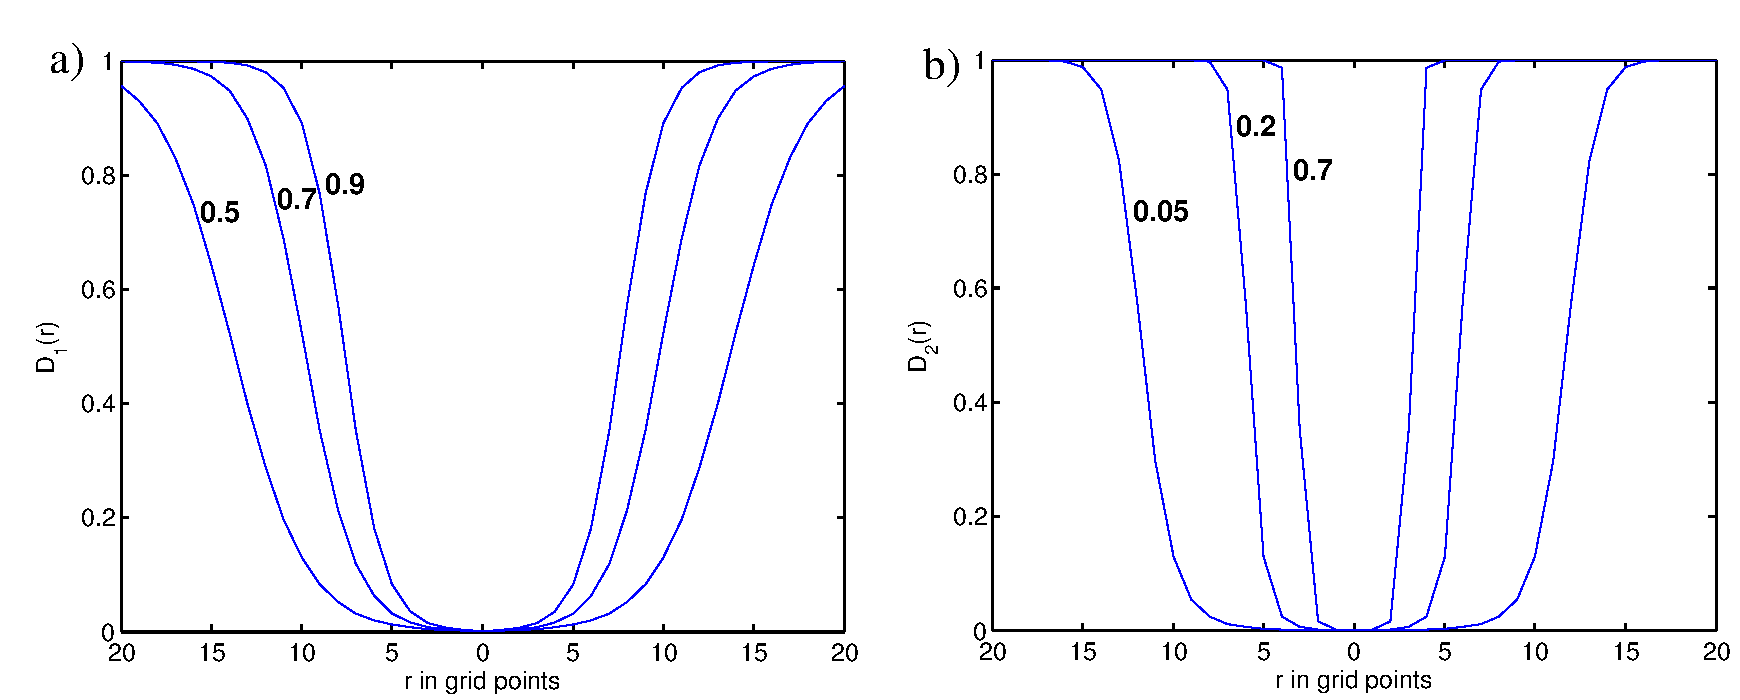
\includegraphics[width=0.8\textwidth]{fig/taper}
\caption[Exemplary taper functions for preconditioning]{Taper functions $D_1$ (a) $D_2$ (b)  with $a=1000$ for a source or receiver located at zero distance plotted for different values of $b$. }\label{fig:taper}
\end{figure}
Three types of local preconditioning are implemented in IFOS3D:\\
- a spherical tapering around source and receiver positions,\\
- a taper around source and receiver planes,  \\
- a taper of the C-PML boundaries\\
The tapering of the C-PML boundaries $D_{PML}(\textbf x)$ is implemented using the $D_2$-function, where the distance to the model boundary is used for $r$. It can be necessary because FWI tends to produce artefacts in the boundary. Using a source taper $D_s$ and a receiver taper $D_r$ the total preconditioned gradient can be estimated as 
\begin{equation} \textbf{p}_k(\textbf x)=D_sD_rD_{PML}\nabla E_k.\end{equation}

\section{Calculation of the conjugate gradient as search direction}
The preconditioned gradient can be used as search direction for updating the model as seen in equation~\ref{equ:update1}. However, the use of the conjugate gradient can stabilise the inversion and improve convergence. The preconditioned gradient of the current iteration ($\textbf p_k$) and the preconditioned gradient ($\textbf p_{k-1}$) and conjugate gradient ($\textbf c_{k-1}$) of the previous iteration are used to calculate the conjugate gradient direction according to the equations~\ref{equ:conjgrad1} and \ref{equ:beta}. Thus, the application of the conjugate gradient method requires the storage of preconditioned gradient and conjugate gradient of the previous iteration.\\
The conjugate gradient gives the direction for the model update, but does not contain information about its size (also with respect to other parameter classes). We therefore normalise  $\textbf c_{k}$ to its maximum and multiply it with a reference value of the respective parameter class ($v_p^0$, $v_s^0$, $\rho^0$): 
\begin{equation}
 c_k^{v_p}(\textbf x)\rightarrow\frac{c_k^{v_p}(\textbf x)}{max(c_k^{v_p}(\textbf x))}v_p^0 \hspace{0.8cm} c_k^{v_s}(\textbf x)\rightarrow\frac{c_k^{v_s}(\textbf x)}{max(c_k^{v_s}(\textbf x))}v_s^0  \hspace{0.8cm} c_k^{\rho}(\textbf x)\rightarrow\frac{c_k^{\rho}(\textbf x)}{max(c_k^{\rho}(\textbf x))}\rho^0 \label{equ:scaled_grad}
\end{equation}
Additionally, a step length estimation is performed as described in the next section.

\section{Step length calculation}\label{sec:steplength}
A good step length calculation is crucial for a good performance in FWI. However, run time for its estimation should be low. IFOS3D uses a parabola  method \citep[e.g.][]{Kur09} to find the optimal step length, which can be achieved at reasonable computational costs. Additionally to the current model misfit the misfit values for two test step lengths are calculated. To mitigate runtime, this is only done for a subset of shots ($N_s$(step)). The three misfit values are used to find a parabola. The location of its minimum is adopted as optimal steplength $\alpha_k$ for the  model update. This results in ($2\times N_s$(step)) additional forward modelings.\\
Of course, the parabola is only a rough approximation of the real misfit curve. Therefore additional condtitions are employed for a successfull steplength estimation:
\begin{enumerate}
 \item in case, the parabola extremum is a maximum, I use the test steplength with the smallest misfit
\item a maximum steplength is defined, which cannot be exceeded
\item if a steplength of zero is estimated or the steplength is negative, the model is updated using a small ratio of the first test-steplength
\end{enumerate}
The choice of the test step length is important for the performance of this method. Generally, the test step length can be larger at the beginning of the inversion, when larger model updates determine the rough structure of the subsurface. Later smaller changes of the model are required for the finer model structures. In IFOS3D an initial test step length (TESTSTEP) is chosen and employed in the first iteration within each frequency band. For later iterations the optimal steplength $\alpha_k$ of the previous iteration is used and the new test step length is determined as $\alpha_k/2$. If the new test step length is larger than TESTSTEP, TESTSTEP is used for the next iteration. If the new test step length is smaller than 25\% of TESTSTEP, it is set to 25\% TESTSTEP.\\
Note, that one steplength is estimated for all parameter classes. It can be useful to limit the update of one parameter class with respect to another. This can be achieved by applying weighting factors in the model update. 
\section{The model update} 
Starting from some starting model the model in each iteration $k$ is updated with $(-\alpha_k\textbf c_k)$.\\
In general, the elastic FWI updates three parameter classes ($v_p$, $v_s$ and $\rho$). The conjugate gradients are calculated for each parameter class and are scaled with an average of this parameter to take into account the size of these parameters with respect to ech other. However, note that only one step length is estimated for all parameters. It can be useful to limit the update of one parameter class with respect to another. This can be achieved by applying additional weighting factors in the model update. 
\section{The full inversion process}
Full waveform inversion is an iterative process. We search for the optimal model by updating the model parameters in the direction of the steepest descent of the misfit function to reach its minimum. However, the inversion of seismic data is generally highly nonlinear and the misfit function is not a smooth function, but contains a lot of local minima. Using a local inversion method like the conjugate gradient approach, it is possible to end up in a local minimum. In this case, the observed data might be explained relatively well by the inverted model, but the model structures are not correct. To find the real subsurface model, the choice of the starting model and different inversion strategies are important.
\subsection{The starting model}
The choice of the starting model is crucial for FWI. The starting model should contain preliminary information about the subsurface, especially for complex data. It can be useful to use a smooth starting model because hard contrasts of interfaces and structures are difficult to change with FWI. The starting model should already approximately explain the low frequency data so that no cycle skipping problems arise. This means, that the required smoothness of the starting model is dependent on the availability of low frequency data.
\subsection{Multi-scale inversion}
It is very helpful not to invert the whole data set at once, but to start with a portion of data and add more data in different stages of the inversion. There are generally three different types for the selection of data:
\begin{enumerate}
 \item frequency filtering: The inversion starts with the inversion of low frequency data and subsequently adds higher frequencies,
 \item time windowing: first arrivals are inverted as a first step, and more data is added in later stages,
 \item offset windowing: seperate long and short offset data
\end{enumerate}
The choice of the inversion strategy depends on the dataset and on the complexity of the problem and a combination of different strategies can be useful. In IFOS3D only the first strategy, the frequency filtering is available at the moment. In the following,
we will explain this method in more detail.
\subsection{Frequency stages}
\begin{figure}[h!]
\begin{center}
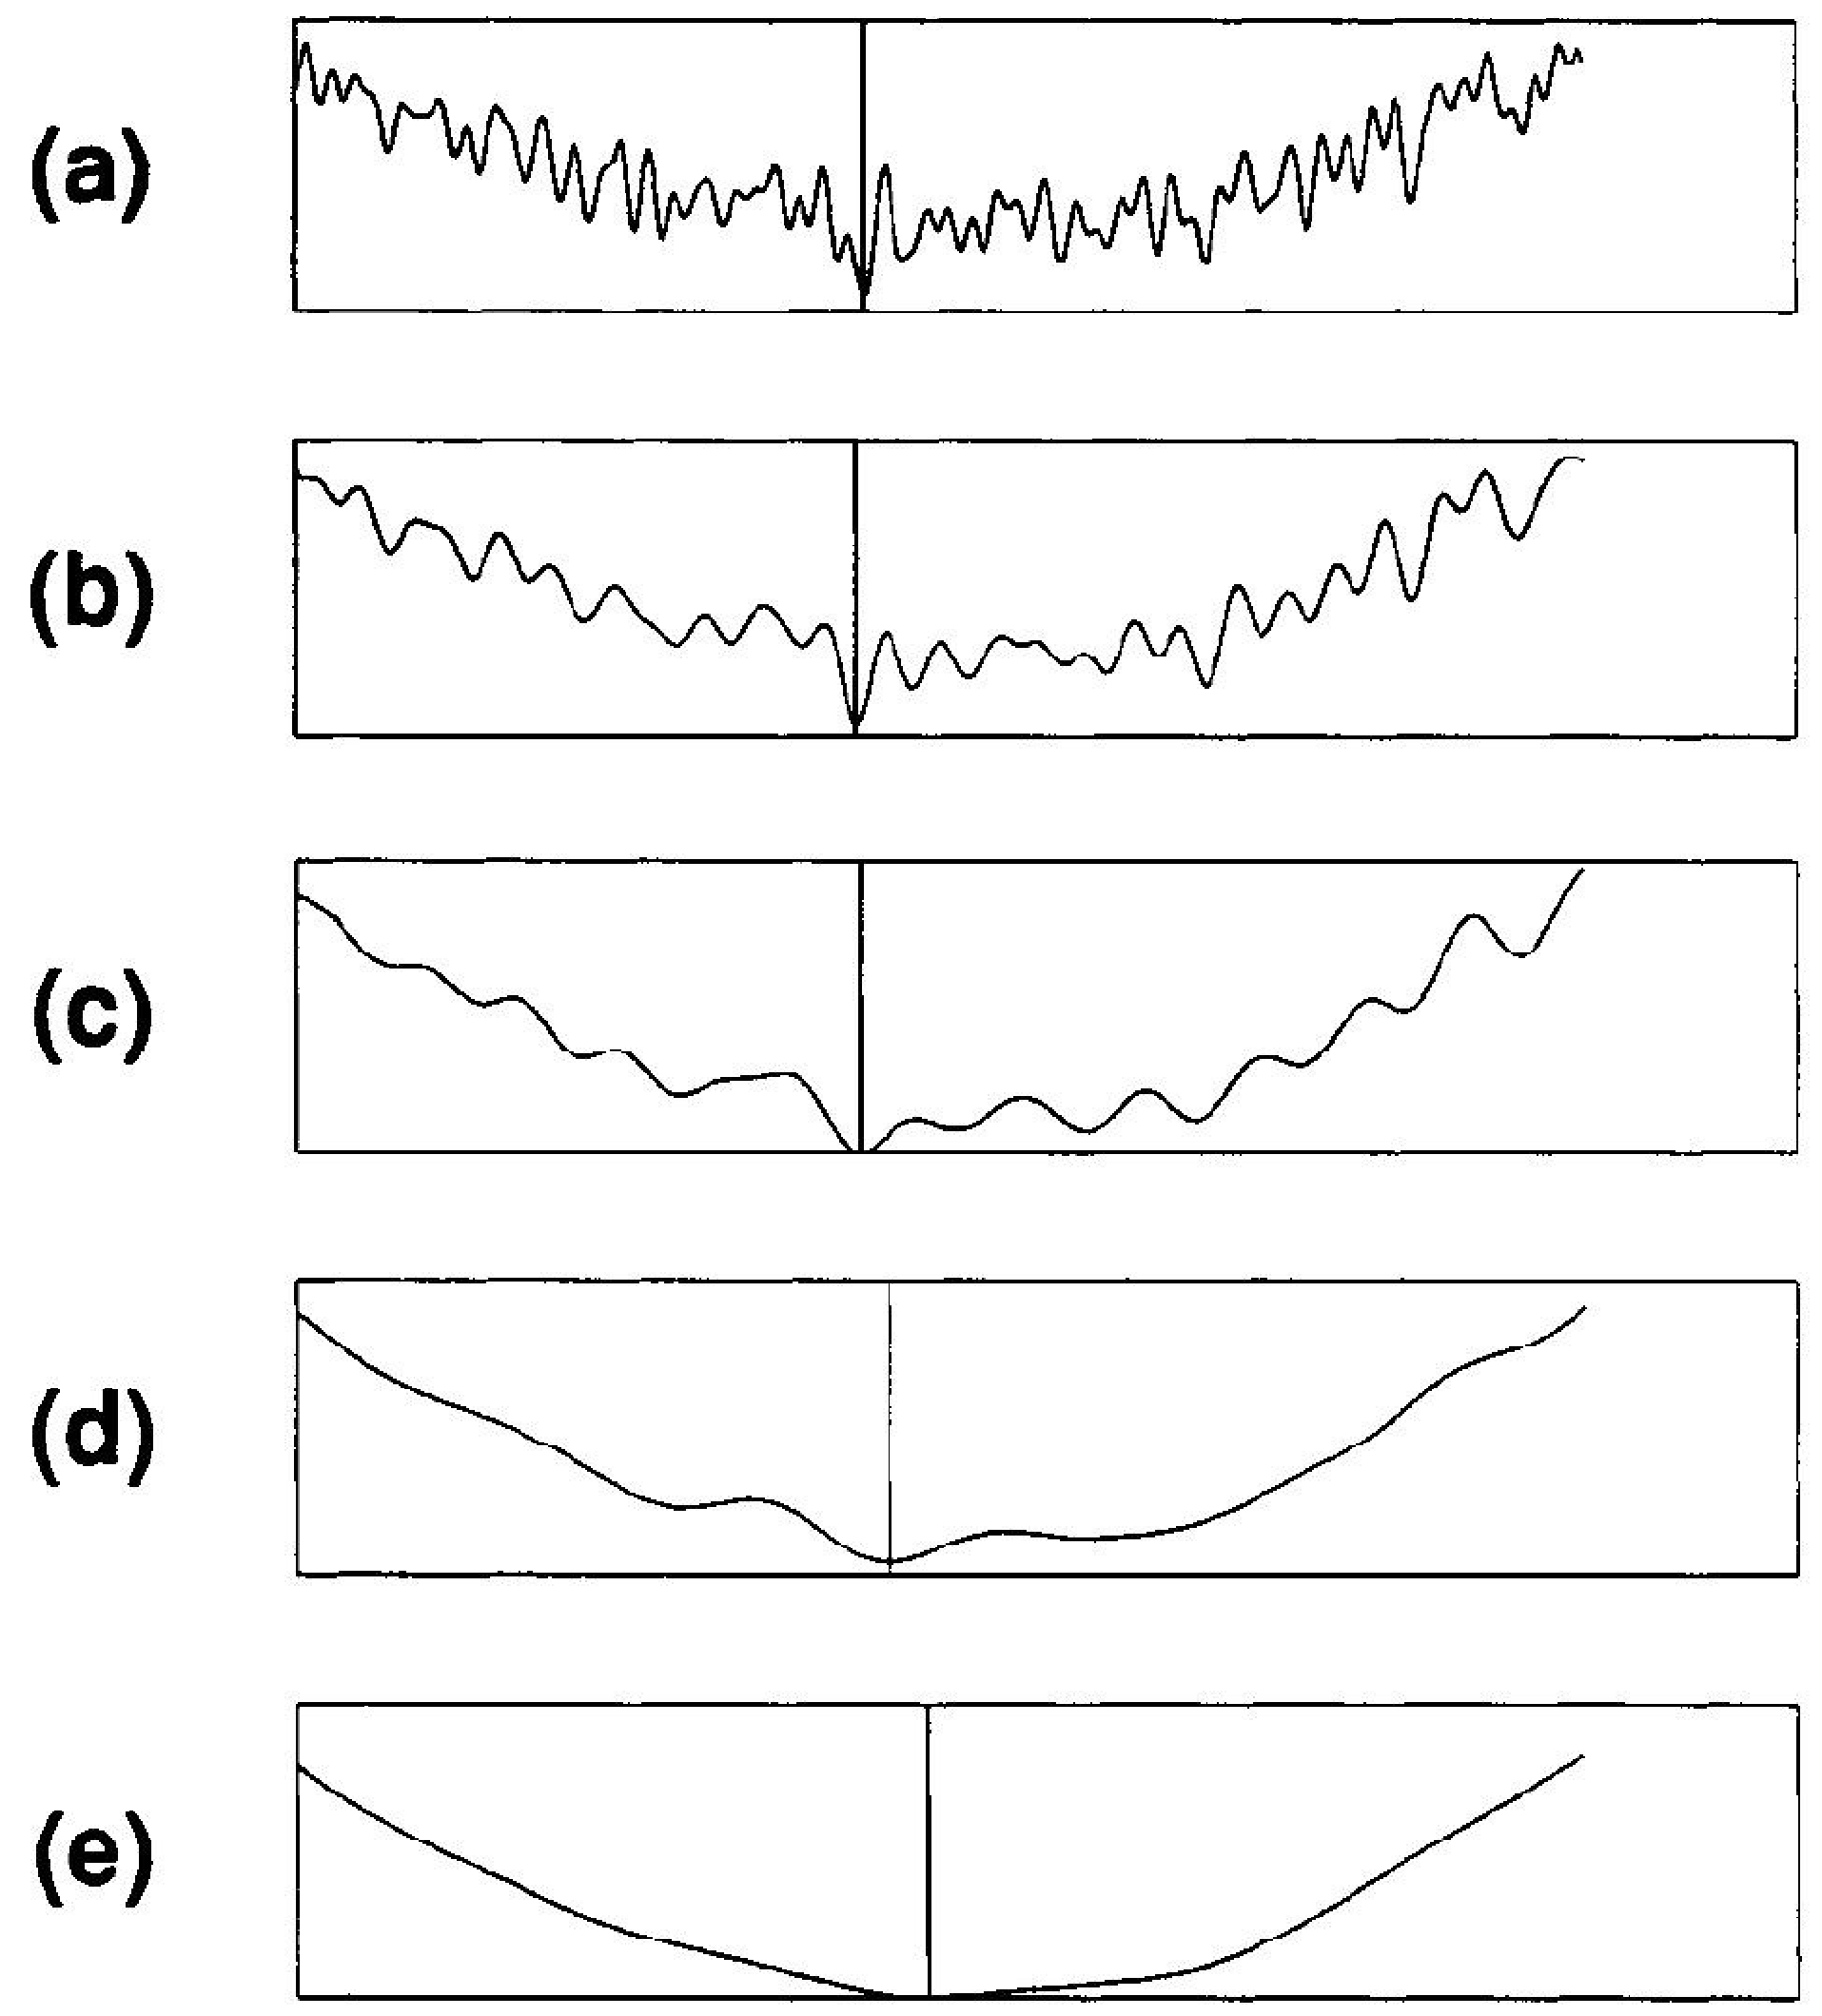
\includegraphics[width=0.5\textwidth]{fig/misfit_bunks}
\caption[Misfit at different scale lengths (from \cite{Bun95})]{Illustration of the misfit function for scale lengths increasing from a) to e) [from: \cite{Bun95}].}\label{fig:bunks}
\end{center}
\end{figure}
IFOS3D calculates the gradient from few monochromatic frequency domain wavefields. Hereby the inversion is subdivided into different frequency stages, which use a different set of frequencies. It is a common technique in FWI to start from low frequencies, to invert for the larger-scaled subsurface structures and then include higher frequencies to find finer model structures. This approach is well demonstrated by Figure~\ref{fig:bunks} from \citep{Bun95}. The misfit function is plotted for different scale lengths, which increase from a) to e). With increasing scale, and thus with decreasing frequency, the misfit function becomes smoother and the number of local minima decreases. Therefore, to reach the global minimum, a model can be much farther away from the real model for low frequencies, whereas a much closer model is required for high frequencies. This can also be understood when looking at the data. Phase differences between the modelled and the observed data need to be smaller than half a period, so that the phases can be assigned correctly to each other. Otherwise cycle skipping can occure and the inversion might end up in a local minimum. This condition is easier to fullfill for lower frequencies. Hence, a multi-scale approach in FWI can mitigate the problem of cycle-skipping and help to reach the global minimum.
\subsubsection*{The choice of frequencies}
There are different ways to include higher frequencies in a multi-scale inversion. \cite{Bro09} tested three different approaches:
\begin{itemize}
\item sequential approach: single frequency inversion using one frequency at a time
 \item Bunks approach: starting from one low frequency, one higher frequency per stage is added, so that the number of frequencies per stage increases
\item simultaneous approach: a group of typically 3-5 frequencies is inverted in each stage, overlapping frequency bands
\end{itemize}
Overall, they found the best performance for the simultaneous inversion of several frequencies, with overlapping frequency bands for their reflection geometry application. Thus, the entrainment of the lower, already inverted frequencies in the Bunks approach does not seem to improve the inversion. \cite{Pra99} also showed an improved performance, when using five instead of three frequencies during one frequency stage. Thus a higher number of frequencies can improve the inversion and a single frequency approach does not seem to be favourable, even though successful applications show that single frequency inversions are possible.\\
Fortunately, the use of frequency groups with few frequencies per stage instead of a single frequency in a time-frequency FWI does not increase the computational costs by much. By contrast when employing a frequency domain forward solver, these frequencies need to be simulated additionally.
\subsubsection*{Frequency intervals}
The choice of the frequency interval needs to ensure a continuous coverage of the wavenumber spectra. \cite{Sir04} showed, that this can generally be fulfilled for frequency intervals larger the sampling interval of $1/T$ ($T$: length of time series), when considering not only one trace but a range of offsets.  Hereby larger offsets enable the coverage of the wavenumber spectra with a lower frequency sampling. For a simple 1D model, the relevant frequencies can be calculated with 
\begin{equation} f_{n+1}=\frac{f_n}{\alpha_{min}},\end{equation}
where $\alpha_{min}$ depends on the offset-to-depth ratio and is smaller for larger maximum offsets \citep{Sir04}.  Still, the use of additional  frequencies increases the redundancy of the data which generally results in improved images, especially in case of higher nonlinearity of the inversion.
\section{Preconditioning with the diagonal Hessian approximation}\label{sec:hess}
In section~\ref{sec:preconditioning} we discussed a very simple method of preconditioning, which locally damps the gradient around sources and receivers. This method works nicely for simple problems as for example often found in transmission geometries. However, in case of complex wavefields this method is not sufficient. If we look at surface geometries, we find that the gradient is very concentrated near the surface, where most energy of the wavefield travels. This means that deeper model parts are not updated without an enhancement by preconditioning. IFOS3D offers the  possibility to employ an approximation of the diagonal Hessian for preconditioning. This approach takes information about the second derivative of the misfit function, the Hessian into account and is a physically funded method. The diagonal elements of the Hessian predict the geometrical amplitude spreading contained in the gradient and can thus be used  to find an improved  spatial scaling of the gradient. In surface seismic, the scaling of the gradient with the diagonal elements of $\textbf H_a$ enhances the influence of deeper parts of the model. In the following we will give an overview about the implementation. For additional information about the role of the Hessian in FWI we refer to \cite{Pra98, Vir09, Bro11} and \cite{But15}.
\subsection{The Hessian operator}
The full Newton method uses the Hessian marix $\textbf H$ for its model update given by
\begin{equation} \delta\textbf m=-\textbf H^{-1}\nabla_mE.\end{equation} In case of a linear inversion problem, an update with $\delta\textbf m$ would lead into the minimum of the misfit function within one step. Non-linear inversion problems, like FWI are linearised step-wise and iteratively approach the minimum. Still the convergence of the Newton method is much improved compared to the gradient methods.
The Hessian is the second derivative of the misfit function with respect to the model parameters:
\begin{equation}H_{jl}=\frac{\partial^2 E(\textbf m)}{\partial m_j\partial m_l} \hspace{0.5cm} (j=1,...n)\hspace{0.2cm}(l=1,...n). \label{equ:hessb}\end{equation}
The variable $n$ denotes the number of model parameters. The size of $\textbf H$ with $n\times n$ is huge and its explicit calculation is therefore very expensive. For large FWI problems like the 3D elastic FWI applications it is not possible. Still the gradient method can be improved by using some information about the Hessian. Comparing the model update of the gradient method (equation~\ref{equ:update1}) with the Newton update, the gradient method approximates $\textbf H$ by $\alpha \textbf P$. By preconditioning the gradient with an approximation of the diagonal Hessian it is thus possible to improve the gradient method.
\subsection{Theory}
\subsubsection*{Calculation of the diagonal Hessian approximation}
The second derivative of the $L_2$-norm based misfit function (equation~\ref{eq:L2}) can be expressed as   \begin{equation}H_{jl}=\sum_{s}\int_0^T dt \sum_{r}\frac{\partial u_i}{\partial m_j}\frac{\partial u_i}{\partial m_l}+R_{jl} =(H_a)_{jl}+R_{jl}.\label{equ:Hess_L2}\end{equation}
In the following we neglect the second term $R_{jl}$ which contains second order partial derivative wavefields and constrain to the first term, the so-called ``approximate Hessian'' $(H_a)_{jl}$. It is calculated as a zero-lag cross-correlation of the first order partial derivative wavefields summed up over all sources $s$ and receivers $r$.\\
For preconditoning in IFOS3D we only use the diagonal elements and calculate the elements $(H_a)_{jj}$ for discrete frequencies. Equation~\ref{equ:Hess_L2} then transforms to \citep{But15}
\begin{equation}(H_a)_{jj}=\sum_{s}\sum_{r}\sum_{v=1}^{nf}\frac{\partial\tilde u_i}{\partial m_j}\left(\frac{\partial\tilde u_i}{\partial m_j}\right )^*. \label{Hess_diag}\end{equation}
The adjoint gradient method does not directly calculate the partial derivative wavefields also known as Fr\'echet derivative kernels which are now required for the estimation of the elements $(H_a)_{jj}$. The derivatives with respect to the elastic parameters $\lambda$, $\mu$ and $\rho$ in frequency domain can be expressed as (see \cite{But15})
\begin{equation}
\begin{split}
 \frac{\partial \tilde u_i(\textbf x_r,\omega_v)}{\partial\rho(\textbf x)} & =\omega_v^2\tilde G_{ji}(\textbf x,\omega_v;\textbf x_r,0)\tilde u_j(\textbf x,\omega_v),\\
\frac{\partial\tilde u_i(\textbf x_r,\omega_v)}{\partial\lambda(\textbf x)} & =-\frac{\partial}{\partial x_j}\tilde G_{ji}(\textbf x,\omega_v;\textbf x_r,0)\frac{\partial\tilde u_p(\textbf x,\omega_v)}{\partial x_p},\\
\frac{\partial\tilde u_i(\textbf x_r,\omega_v)}{\partial\mu(\textbf x)} & =-\frac{1}{2}\left (\frac{\partial}{\partial x_k}\tilde G_{ji}(\textbf x,\omega_v;\textbf x_r,0)+\frac{\partial}{\partial x_j}\tilde G_{ki}(\textbf x,\omega_v;\textbf x_r,0)\right )\left (\frac{\partial\tilde u_j(\textbf x,\omega_v)}{\partial x_k}+\frac{\partial\tilde u_k(\textbf x,\omega_v)}{\partial x_j}\right ).
\end{split}\label{equ:frechet4}
\end{equation}
The terms $\tilde G_{ji}(\textbf x,\omega_v;\textbf x_r,0)$ denote the Green's receiver functions for discrete frequencies, which are multiplied with the forward wavefields. Same as for the gradient calculation we transform these equations to the seismic velocity parametrisation by using the chain rule
 \begin{equation}
\begin{split}
 \frac{\partial\tilde u_i}{\partial v_p}& =2\rho v_p\frac{\partial\tilde u_i}{\partial\lambda},
\\
\frac{\partial\tilde u_i}{\partial v_s}& = -4\rho v_s\frac{\partial\tilde u_i}{\partial\lambda}+2\rho v_s\frac{\partial\tilde u_i}{\partial\mu},
\\
\frac{\partial\tilde u_i}{\partial\rho'}& = (v_p^2-2v_s^2)\frac{\partial\tilde u_i}{\partial\lambda}+v_s^2\frac{\partial\tilde u_i}{\partial\mu}+\frac{\partial\tilde u_i}{\partial\rho}.
\end{split}\label{equ:partial_wave2}
\end{equation}
Finally these partial derivative wavefields can be used for the estimation of the diagonal Hessian approximation $H_a^{v_p}(\textbf x)$, $H_a^{v_s}(\textbf x)$ and $H_a^{\rho'}(\textbf x)$ (equation~\ref{Hess_diag}).
\subsubsection*{Hessian preconditioning}
As preconditioning operator ($P^\rho(\textbf x)$, $P^\lambda(\textbf x)$ and $P^\mu(\textbf x)$) for the different parameters we use the inverse of the diagonal of $\textbf H_a$, which is straightforward for a diagonal matrix:
\begin{equation}
 \begin{split}
 P^\rho(\textbf x) & = (H_a^\rho(\textbf x)+\epsilon_\rho)^{-1},\\
 P^{v_p}(\textbf x) & = (H_a^{v_p}(\textbf x)+\epsilon_{v_p})^{-1},\\
 P^{v_s}(\textbf x) & = (H_a^{v_s}(\textbf x)+\epsilon_{v_s})^{-1}.
\end{split}\label{Hess_precon}
\end{equation}
The coefficients $\epsilon_\rho$, $\epsilon_\lambda$ and $\epsilon_\mu$ are water levels, which are summed to the Hessian approximations for reasons of stability. Otherwise, very small elements of $\textbf H_a$ in areas of very low wave coverage cause a strong increase of the gradient in these areas which can result in artefacts.
\subsection{Implementation of Hessian preconditioning}
The implementation of Hessian preconditioning in IFOS3D is illustrated in figure~\ref{fig:workflow_hess}. Note, that the Hessian computation depends on the acqusition geometry and the current model $\textbf m_k$ but does not contain information about the true subsurface model.
\begin{figure}[h!]
\begin{center}
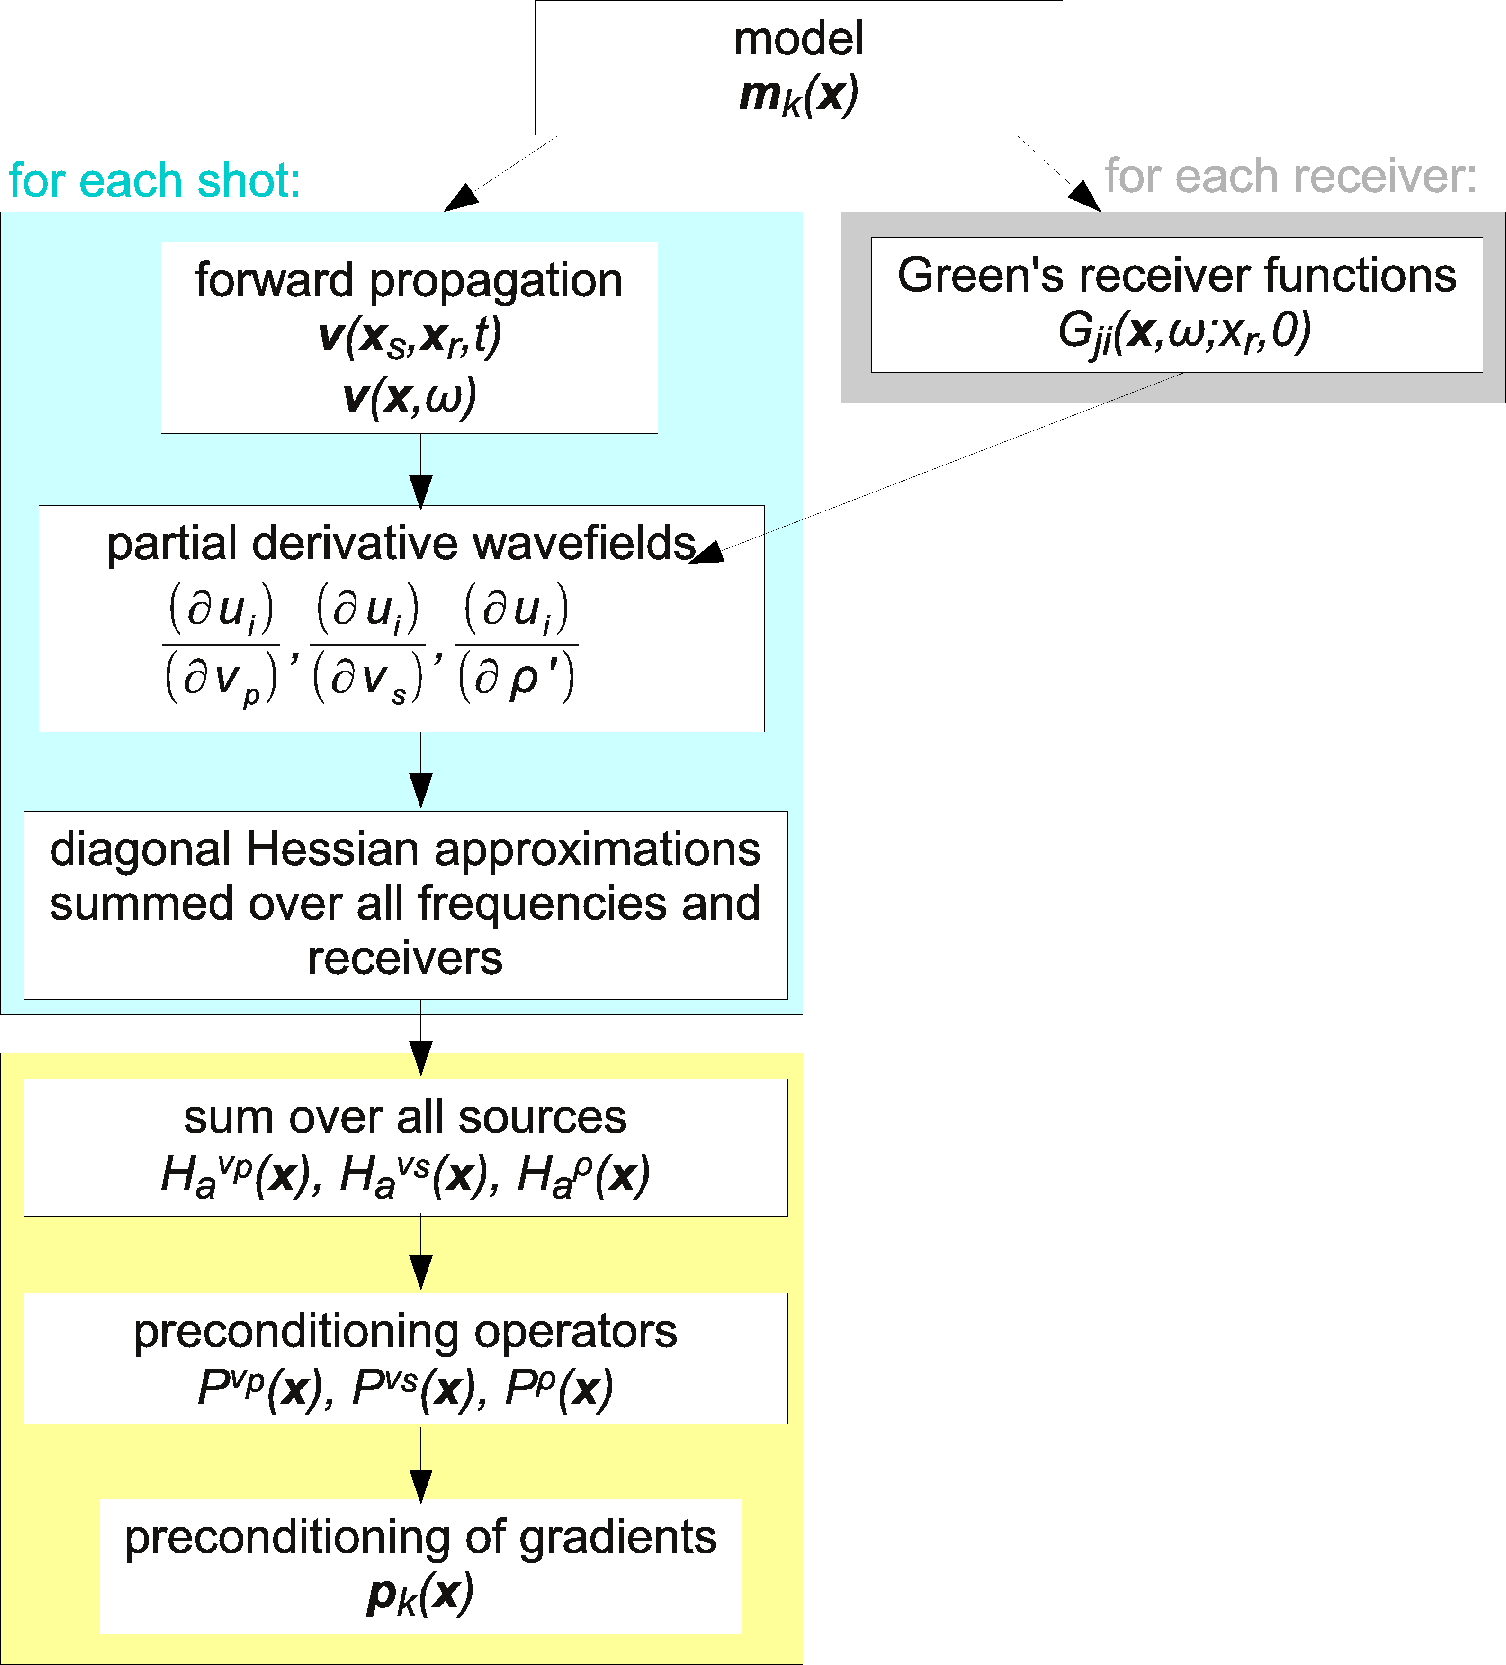
\includegraphics[width=0.75\textwidth]{fig/workflow_hess_22}
\caption[Workflow for the calculation of the Hessian preconditioning operator]{Workflow for the calculation of the Hessian preconditioning operator at iteration $k$ as implemented in IFOS3D.}\label{fig:workflow_hess}
\end{center}
\end{figure}
\subsubsection*{Wavefield calculation}
The forward propagation of wavefields and the extraction of monochromatic frequency wavefields ($\textbf v(\textbf x,\omega$)) is already performed in the framework of the gradient calculation (section~\ref{sec:grad_calc}). The main additional computational effort is spend for the computation of the Green's receiver functions $\tilde G_{ji}(\textbf x,\omega_v;\textbf x_r,0)$. Differently to the gradient calculation, where the backpropagated wavefield is propagated from all receivers simultanously, the complete set of Green's receiver functions requires one propagation for each receiver and each component, resulting in $3\times N_{rec}$ additional wavefield simulations ($N_{rec}$: total number of receivers). We calculate the Green's receiver functions for displacement by using a Heaviside step function ($\Theta$) as a force-time function, defined as 
$$\Theta(t-t_{step})=
 \begin{cases}
  0 \mbox{ for } t<t_{step}\\
1\mbox{ for } t\geq t_{step},
 \end{cases}$$
with the $\delta(t-t_{step})$-function as its derivative. The same time shift $t_{step}$ is used for the forward source. To estimate the Green's receiver functions in frequency domain, we apply a discrete Fourier transform (equation~\ref{equ:discFourier}) to the function $G_{ij}(\textbf x_r,t;\textbf x,t_{step})$ on the fly. The functions $G_{ij}(\textbf x_r,\omega_v;\textbf x,0)$ are stored in memory for each discrete frequency and each receiver. Due to the high computational runtime and storage demand, we employ two approximations here. Firstly, we only use a subset of receivers. Secondly, we only calculate the component of the Green's receiver functions which corresponds to the source of the forward wavefield and thus calculate only one component of the partial derivative wavefield. These limitations have only small effects on the gradient corrections near the source, where preconditioning is most important. However, an additional local preconditioning of the smaller receiver artefacts becomes necessary. 
\subsubsection*{Hessian calculation}
For each shot the partial derivative wavefields are computed by multiplying the forward field with each Green's receiver function for each frequency according to equations~\ref{equ:frechet4} and \ref{equ:partial_wave2}. Hereby, the velocities of the forward wavefield are integrated with $(i\omega)^{-1}$ to find the displacement fields and spatial derivatives are calculated with finite differences of fourth order. The partial derivative wavefields are multiplied with their complex conjugate and summed up over all frequencies and receivers and finally over all shots to find the diagonal Hessian approximation for $v_p$, $v_s$ and $\rho$ (equation~\ref{Hess_diag}). 
\subsubsection*{Preconditioning}
Finally, the preconditioning operator can be calculated according to equation~\ref{Hess_precon} and applied to the gradient ($\textbf P(\textbf x) \nabla E_k$). At the moment no automatic estimation of the water levels $\epsilon$ is implemented and the water levels are taken from the input file. Thus an empirical try of $\epsilon$ and its effects on the gradient preconditioning is required using the gradient and Hessian of the current iteration.\\
An additional local damping of the gradient around the receiver positions and in the C-PML boundaries is applied.
\subsubsection*{The full inversion process}
The Hessian preconditioning operator is calculated once at the beginning of each frequency stage. It is applied throughout this stage. Unfortunately, the estimation of the water level $\epsilon$ is not automised at the moment. That means, that in practice before the inversion starts a new frequency stage, the gradient and Hessian are estimated and the water level is determined empirically. This results in as additional calculation of the first gradient of each frequency stage.\\
Apart from the calculation and application of the Hessian preconditioning operator the inversion process, like gradient normalisation, model update and steplength calculation remains unchanged. 
\subsubsection*{Costs of Hessian preconditioning}
The Hessian preconditioning operator is calculated once per frequency stage. The main extra run time is spend for the modelings of the Green's receiver functions which number corresponds to the subset of receivers used for these calculations. Additionally, one extra gradient computation is performed as long as the empirical determination of $\epsilon$ before each frequency stage is required.\\
In summary, the following approximations are made compared to the use of the full Hessian matrix:
\begin{itemize}
 \item use of diagonal elements of $\textbf H_a$ only,
\item employ only a subset of receivers for its calculation,
\item only one component of partial derivative wavefields by  backpropagating only one component $\delta$-pulse and
\item estimate Hessian only once for each frequency stage.
\end{itemize}

\section{The L-BFGS method}\label{sec:lbfgs}
This section introduces the L-BFGS (low memory BFGS) method, named after the BFGS-method developers, i.e. Broyden, Fletcher, Goldfarb and Shannon. The method belongs to the class of the quasi-Newton methods and is implemented in IFOS3D as an optimisation of the inversion process. The Hessian operator and Newton methods were shortly explained in the previous chapter. Instead of calculating the inverse Hessian $\textbf H_k^{-1}$ directly, quasi-Newton methods approximate the (inverse) Hessian by using the change of the gradients over the iterations. Starting from an initial Hessian approximation $\textbf H_0$ the approximation of the (inverse) Hessian is updated in each iteration to find a more accurate estimate for the Hessian. \\
The application of the inverse Hessian to the gradient acts as deconvolution of the gradient from limited-bandwidth effects and geometric amplitude effects \citep{Pra98,Bro09}. Previous applications for 2D FWI by \cite{Bro09} and \cite{Bro11} showed higher convergence rates and sharper images when using the L-BFGS approach compared to the conventional conjugate gradient method. Additionally, a correct inversion of multiple parameter classes can be achieved which requires no empirical weighting of the different parameter classes.
\subsection{Theory of the BFGS and L-BFGS method}
Using the changes of the gradients $\pmb{\gamma}_k=\nabla E_{k+1}-\nabla E_{k}$ and the model changes $\textbf s_k=\textbf{m}_{k+1}-\textbf{m}_{k}$ the BFGS-condition is formulated as \citep{Noc99}
\begin{equation}
 \textbf{H}_{k+1}^{-1}=\textbf V_k^T\textbf H_k^{-1}\textbf V_k+r_k\textbf s_k\textbf s_k^T \hspace{0.5cm} \text{with} \hspace{0.2cm} r_k=\frac{1}{\pmb{\gamma}_k^T\textbf s_k}  \hspace{0.5cm} \text{and} \hspace{0.2cm}\textbf V_k=\textbf I-r_k\pmb{\gamma}_k\textbf s_k^T.\label{equ:BFGS}
\end{equation}
The inverse Hessian approximation is updated in each iteration starting from an initial guess $\textbf H_0^{-1}$ without explicitely calculating the second derivatives. However, it is not suitable for a large number $n$ of model parameters due to the huge size of the Hessian matrix ($n\times n$).\\
By contrast, the L-BFGS method does not explicitely store the Hessian matrix, but uses changes in gradient and model of only the recent $m$ iterations and calculates the inverse Hessian newly in each iteration. Applying equation~\ref{equ:BFGS} repeatedly for the previous $m$ iterations results in the following formula \citep{Noc99}:
\begin{equation}
 \begin{split}
  \textbf H_k^{-1}=& (\textbf V_{k-1}^T...\textbf V_{k-m}^T)\textbf H_{k0}^{-1}(\textbf V_{k-m}...\textbf V_{k-1})\\
      & +r_{k-m}(\textbf V_{k-1}^T...\textbf V_{k-m+1}^T)\textbf s_{k-m}\textbf s_{k-m}^T(\textbf V_{k-m+1}...\textbf V_{k-1})\\
      & +r_{k-m+1}(\textbf V_{k-1}^T...\textbf V_{k-m+2}^T)\textbf s_{k-m+1}\textbf s_{k-m+1}^T(\textbf V_{k-m+2}...\textbf V_{k-1})\\
      & +... \\
      & +r_{k-1}\textbf s_{k-1}\textbf s_{k-1}^T.
 \end{split}\label{equ:LBFGS}
\end{equation}
$\textbf H_{k0}^{-1}$ is an initial inverse Hessian approximation, which is allowed to vary from iteration to iteration.
\subsection{The L-BFGS update}
The L-BFGS method can be implemented very efficiently in FWI. In IFOS3D we apply the recursive algorithm described by \cite{Noc99} which estimates the product $\textbf H_k^{-1}\nabla E_k$ without forming the inverse Hessian approximation directly. It can be written as \vspace{0.5cm}\\
\line(1,0){125}\\
$\textbf q \leftarrow \nabla E_k$\\
\textbf{for} ($i=k-1,...,k-m$)\\
$\hspace*{1cm} \alpha_i \leftarrow r_i\textbf s_i^T\textbf q$\\
\hspace*{1cm} $\textbf q\leftarrow\textbf q-\alpha_i\pmb{\gamma}_i$\\
\textbf{end for}\\
$\textbf z \leftarrow \textbf H_{k0}^{-1}\textbf q$\\
\textbf{for} ($i=k-m,...k-1$)\\
\hspace*{1cm}$\beta\leftarrow r_i\pmb{\gamma}_i^T\textbf z$\\
\hspace*{1cm}$\textbf z\leftarrow\textbf z+\textbf s_i(\alpha_i-\beta)$\\
\textbf{end for}\\
$\textbf H_k^{-1}\nabla E_k=\textbf z$\\
\line(1,0){125}\vspace{0.5cm}\\
This algorithm is performed once in each iteration and consists of $(4mn+n)$ multiplications if a diagonal $\textbf H_{k0}^{-1}$ is chosen. The L-BFGS algorithm requires additional storage of $(2mn+m)$ floating numbers for $\pmb\gamma, \textbf s$ and $r$. For reasonable numbers of $m$ the L-BFGS method can therefore be performed at relatively low extra costs of runtime an storage. In general, values between 5 and 20 are used for $m$. In the first $(m-1)$ iterations the result corresponds to the BFGS method. 
\subsection{The optimised FWI workflow}
\subsubsection{Hessian preconditioning and L-BFGS}
Following the approach by \cite{Bro11} we apply the L-BFGS method by using changes in gradients preconditioned by the diagonal Hessian approximation. The Hessian preconditioning (section~\ref{sec:hess}) already offers an improved scaling of the gradient. By additionally using the L-BFGS algorithm, the off-diagonal elements of the gradient are taken into account. Furthermore, the L-BFGS method is calculated in each iteration, whereas the diagonal Hessian matrix is estimated only once per frequency stage. When using the preconditioned gradients a scaled identity matrix \citep{Noc99} is sufficient as initial guess for the Hessian:
\begin{equation} \textbf H_{k0}^{-1}=\frac{\textbf s_{k-1}^T\pmb{\gamma}_{k-1}}{\pmb{\gamma}_{k-1}\pmb{\gamma}_{k-1}^T}\textbf I,  \end{equation}
\subsubsection*{Parameter normalisation}
The conjugate gradient does not offer information about the update of the different model parameters with respect to each other. This is changed when taking the off-diagonal elements of the Hessian into account. The L-BFGS method can thus improve the multi-parameter inversion by adding information about off-diagonal elements of the Hessian. To achieve a dimensionless L-BFGS sheme for the different parameter classes we normalise the inversion sheme with some representative model parameters $v_{p0}, v_{s0}$ and $\rho_{0}$ as suggested by \cite{Bro11} with   
\begin{equation}
 \hat v_p(\textbf x)=\frac{v_p(\textbf x)}{v_{p0}}, \hspace{0.5cm}\hat v_s(\textbf x)=\frac{v_s(\textbf x)}{v_{s0}}, \hspace{0.5cm}\hat \rho(\textbf x)=\frac{\rho(\textbf x)}{\rho_{0}}. 
\end{equation}
This leads to a normalisation of the gradients calculated as
\begin{equation}
 \frac{\partial E}{\partial\hat v_p(\textbf x)}=\frac{\partial E}{\partial v_p(\textbf x)}v_{p0},\hspace{0.8cm}\frac{\partial E}{\partial\hat v_s(\textbf x)}=\frac{\partial E}{\partial v_s(\textbf x)}v_{s0},\hspace{0.8cm}\frac{\partial E}{\partial\hat\rho(\textbf x)}=\frac{\partial E}{\partial \rho(\textbf x)}\rho_0
\end{equation}
and a normalisation of the Hessian approximation given by
\begin{equation}
 H_a^{\hat v_p}=H_a^{v_p}v_{p0}^2, \hspace{0.8cm} H_a^{\hat v_p}=H_a^{v_p}v_{p0}^2, \hspace{0.8cm} H_a^{\hat \rho}=H_a^{\rho}\rho_0^2.
\end{equation}
The L-BFGS algorithm calculates a normalised model update, which needs to be denormalised by multiplication with the representative model parameters:
\begin{equation}
\delta v_p=\delta\hat v_p v_{p0}, \hspace{0.8cm} \delta v_s=\delta\hat v_s v_{s0}, \hspace{0.8cm} \delta\rho=\delta\hat\rho\rho_0.
\end{equation}
This dimensionless inversion sheme enables a simultanous L-BFGS algorithm for all parameter classes.
\subsubsection*{Workflow overview}
The workflow of the optimised FWI inversion can be described as follows:\vspace{0.5cm}\\
\line(1,0){125}\\
\textbf{for each frequency stage}
\begin{itemize}
 \item calculate diagonal Hessian approximation ($H_a^{\hat v_p}, H_a^{\hat v_s}, H_a^{\hat\rho}$) for normalised parameters
\end{itemize}
\textbf{in each iteration}
\begin{itemize}
\item calculate gradients of normalised parameters
\item apply diagonal Hessian approximation to gradient 
\item save change in preconditioned gradients and models, discard iterations smaller k-m
\item L-BFGS algorithm to find normalised model update
\item denormalise model update
\item step length calculation: try steplength $\alpha=1$ first
\item model update
\end{itemize}
\line(1,0){125}\\
Newton methods in general calculate an absolute model update and for a linearised Newton method steplenghts close to one are expected. This is also the case for the quasi-Newton L-BFGS sheme. If a good approximation of the Hessian can be achieved  a steplength close to one will be favourable. It is possible to apply a steplength estimation as described in section~\ref{sec:steplength} with a test step length of 0.5 and 1. If the L-BFGS sheme works well, a steplength close to 1 will be estimated after a few iterations. Note, that in the first iteration the inversion corresponds to a gradient method with Hessian preconditioning.


\clearpage
\chapter{Getting started}
\label{Gettingstarted}
\section{Requirements}
\label{requirements}
IFOS3D was tested on different Linux platforms. To run IFOS3D an MPI implementation (one of the three listed below) and a C-Compiler is required.
The code was tested on our local workstation cluster using Suse Linux and OpenMPI. Additionally applications were performed on the JUROPA and JURECA supercomputers in Juelich (Germany) and the Hermit supercomputer at HLRS in Stuttgart (Germany). The following programs should be installed on you machine for a proper run and processing of data. These requirements are similar to the forward solver SOFI3D.

\begin{center}
% use packages: array
\begin{small}
\begin{tabular}{lll}
Program & Description & Weblink \\ 
OpenMPI & MPI Implementation & \url{http://www.open-mpi.org} \\
 & (for the parallelization) & \\
MPICH2 & MPI Implementation & \tiny{\url{http://www.mcs.anl.gov/research/projects/mpich2}} \\ 
& (for the parallelization) & \\
LAM/MPI & MPI Implementation & \url{http://www.lam-mpi.org} \\
& (for the parallelization) & \\
C-Compiler & the whole code is written in C,& \\
& any C-Compiler should be able & \\
& to compile it & \\
Seismic Un*x & Seismic processing package, & \url{http://www.cwp.mines.edu/cwpcodes} \\
(SU)  & SOFI3D outputs seismic data & \\
& in the SU format & \\
Matlab & Preferred program package for & \url{http://www.mathworks.de} \\
(commercial)& the visualization of snapshots, also  & \\
& useful for the display and & \\
& processing of seismograms & \\
xmovie & Console based movie program, can & usually included in Linux distribution\\
& be used for the quick display & otherwise install from repository\\
& of snapshot data  &
\end{tabular}
\end{small}
\end{center}
\section{Installation - The folder structure}
After unpacking the software package (e.g. by  \textbf{tar -zxvf ifos3D.tgz}) and changing to the directory ifos3D ( \textbf{cd ifos3D})  you will find different subdirectories:\vspace{0.2cm}\\
\textbf{bin}\\
This directory contains all executable programs, like ifos3D and snapmerge. These executables are generated using the command  \textbf{make $<$program$>$} (see below).\vspace{0.2cm}\\
\textbf{doc}\\
This directory contains documentation on the software (this users guide). \vspace{0.2cm}\\ 
\textbf{mfiles}\\
Here some Matlab routines (m-files) are stored. They can be used vor processing and visualisation of data. \vspace{0.2cm}\\
\textbf{par}\\
This directory contains the following folders:
\begin{itemize}
 \item \textbf{in\_and\_out}: contains in- and outputfiles of IFOS3D parameters
 \item \textbf{sources}: source parameters
 \item \textbf{receiver}: receiver locations
 \item \textbf{su}: seismogram outputfiles
 \item \textbf{su\_obs}: observed seismograms
 \item \textbf{model}: model in- and output
 \item \textbf{grad}: gradient output
 \item \textbf{hess}: diagonal hessian in- and output
\end{itemize}\vspace{0.2cm}
\textbf{scripts}\\
Here, you will find examples of script-files used to submit modeling jobs on cluster-computers.\vspace{0.2cm}\\
\textbf{src}\\ 
This directory contains the complete source codes. The different subprograms are listed in appendix~\ref{sec:code_overview}.\vspace{0.2cm}\\
\textbf{libcseife}\\
The libcseife library serves for filtering seismograms
\section{Compilation}
To compile ifos3D change to the \textit{par}-directory and perform \textbf{make}. The Makefile will first compile the external libseife library and then compile the main program. In some cases it's necessary to  remove the *.d files in the \textit{libseife}-directory. If problems with the compilation arise go to the \textit{libseife}-directory open \textit{Makefile} and adjust the compiler options for your system.\\
To change the compiler options open the \textit{Makefile} in \textit{src}-directory. Here you can also find examples for compiler options on different systems where IFOS3D or SOFI3D were used in the past.
\section{Running IFOS3D}
To start the program with OpenMPI you can use the command\\
\textbf{mpirun -np 8 nice -19 ../bin/ifos3D ./in\_and\_out/ifOS3D\_toy.json $\mid$ tee ./in\_and\_out/ifos3D.out}\\
which runs IFOS3D on 8 processors with lowest priority. The standard output is written to \textit{/in\_and\_out/ifos3D.out}. You can also use the shell-script \textit{par/startIFOS3D.sh}.\\
For 3D FWI applications it is often useful to use supercomputers in high performance computing centers. Some examples for job scripts can be found in the directory \textit{scripts}.

\clearpage
\chapter{In- and output}
\section{The input file - *.json}
In the following we will describe the input parameters of IFOS3D. The verbatim text shows, how they appear in \textit{in\_and\_out/ifos3d\_inv\_all\_parameters.json}. There is also a commented json file: \textit{in\_and\_out/ifos3d\_inv\_all\_parameters\_commented.json}. The parameters used for the wavefield simulation mostly resemble the parameters of SOFI3D and are also described in the SOFI manual.
\subsection{The grid and its decomposition}
\subsubsection*{The grid}
\begin{verbatim}
"Note that y denotes the vertical direction !" : "comment",
"3-D Grid" : "comment",
			"NX" : "160",
			"NY" : "184",
			"NZ" : "160",
			"DX" : "0.8",
			"DY" : "0.8",
			"DZ" : "0.8",
\end{verbatim}
The cartesian grid system is specified by the number of grid points in each direction (\textbf{NX, NY, NZ}) and by the distance between grid points \textbf{DX, DY, DZ} chosen in the input file. Hereby \textbf{NY} and \textbf{DY} denote the vertical direction! 
The grid spacing needs to satisfy the dispersion criterion at least up to the maximum frequency and minimum wavelength used in the inversion. In case the dispersion criterion is violated for the frequency range of the source wavelet, a warning is given at the beginning of the simulation. The dispersion criterions are given in the SOFI3D manual.
\subsubsection*{Domain decomposition}
\begin{verbatim}
"Domain Decomposition" : "comment",
			"NPROCX" : "2",
			"NPROCY" : "2",
			"NPROCZ" : "2",
\end{verbatim}


The parallelisation is based on domain decomposition. Each processor performs the FWI algorithm for a small subvolume of the total grid system. \textbf{NPROCX}, \textbf{NPROCY} and \textbf{NPROCZ} define the number of processors in each direction, which gives a total number of $NPROCX\times NPROCY\times NPROCZ$ processors. Note, that the number of processors in each direction needs to be a common factor of the number of grid points in this direction.

\subsection{FD-modeling parameters}
\subsubsection*{Order of FD operator}
\begin{verbatim}
"FD order" : "comment",
			"FDORDER" : "4",
			"FDCOEFF" : "2",
\end{verbatim}

The order of the spatial FD-sheme,  which is used for the stress and velocity updates can be chosen as \textbf{FDORDER}=2, 4, 6, 8, 10, and 12. 
These orders result in different dispersion and stability criterions (section~\ref{sec:SOFI3Dcharacter}). A larger FD-order enables a larger grid spacing, however in case of strong heterogeneities a smaller FD-operatot is more accurate. 
With the option \textbf{FDCOEFF} the user can switch between Taylor (\textbf{FDCOEFF}=1) and Holberg (\textbf{FDCOEFF}=2) FD coefficients. Within the CPML boundary a fourth order operator is applied automatically. 
We also use fourth order operators to calculate the spatial derivatives of the wavefield velocity, which are needed for the gradient calculation. IFOS3D uses a second order time discretisation.
\subsubsection*{Time Stepping}
\begin{verbatim}
"Time Stepping" : "comment",
			"TIME" : "0.06",
			"DT" : "5.0e-05",
\end{verbatim}

\textbf{TIME} defines the total simulation length.  The time stepping \textbf{DT} must be chosen to satisfy the stability criterion (SOFI3D  maunual) and thus depends on the grid spacing and the maximum velocity. 
In case of violation IFOS3D will give a warning and terminate. The number of timesteps of the inversion is given by $TIME/DT$.

\subsection{Sources}
\begin{verbatim}
"Source" : "comment",
			"SOURCE_SHAPE" : "4",
			"SOURCE_TYPE" : "4",
			"ALPHA" : "45.0",
			"BETA" : "45.0",
			"SIGNAL_FILE" : "./STF/stf.su",
			"SRCREC" : "1",
			"SOURCE_FILE" : "./sources/sources_toy.dat",
			"RUN_MULTIPLE_SHOTS" : "1",
\end{verbatim}

\subsubsection*{The wavelet}
Different wavelets for the modeling can be chosen:
\begin{itemize}
 \item \textbf{SOURCE\_SHAPE}=1: Ricker wavelet:\\ $s=(1.0-2.0\tau ^2)\text{exp}(-\tau ^2); \hspace{0.5cm}	\tau=\pi f_c(t-1.5/f_c-t_d);$	
\item \textbf{SOURCE\_SHAPE}=2: Fuchs-M\"uller wavelet:\\ $s(t)=\text{sin}(2.0\pi (t-t_d)f_c-0.5 \text{sin}(4.0\pi (t-t_d)f_c); \hspace{0.2cm}\text{for}\hspace{0.2cm}(t_d<t<t_d+1/f_c) \hspace{0.4cm}\text{else}\hspace{0.2cm} s(t)=0$
\item \textbf{SOURCE\_SHAPE}=4: sin$^3$-wavelet:\\ $s(t)=0.75\pi f_c\text{sin}(\pi f_c(t-t_d)^3;\hspace{0.2cm}\text{for}\hspace{0.2cm}(t_d<t<t_d+1/f_c) \hspace{0.5cm}\text{else}\hspace{0.2cm} s(t)=0$
\item \textbf{SOURCE\_SHAPE}=5: step function:\\ $s(t)=0.0; \hspace{0.2cm}\text{if}\hspace{0.2cm}(t<t_d) \hspace{0.5cm}\text{else} \hspace{0.2cm} s(t)=1.0; $
\end{itemize}
The employed center frequency $f_c$ and the time delay of the source wavelet $t_d$ are defined in the source file. An exemplary plot of the different wavelets and the corresponding spectra can be seen in the SOFI3D manual. 
Note, that the symmetric Ricker wavelet is delayed and its maximum period is excited at the source location after one period. The step function is used for the calculation of the diagonal Hessian approximation. \\
If you want to define your own wavelet, you can include this either in the source code in \textit{src/wavelet.c} or use \textbf{SOURCE\_SHAPE}=3 and read in an external wavelet from \textbf{SIGNAL\_FILE}. 
This file should contain the source signal in ASCII with the correct time sampling and with one sample per line, like \\
----------------\\
0.0\\
0.01\\
0.03\\
...\\
----------------
\subsubsection*{The source type}
You can either choose an explosive source (\textbf{SOURCE\_TYPE}=1) exciting compressional waves or a  point force directed in $x$, $y$ (vertical) or $z$  (\textbf{SOURCE\_TYPE}=2,3,4) direction. With \textbf{SOURCE\_TYPE}=5 it is also possible to define a force in arbitrary direction by using the angles \textbf{ALPHA} and \textbf{BETA}. This is illustrated in the SOFI manual. 
The plane wave excitation (\textbf{SOURCE\_REC}=2) was not yet tested for inversion in IFOS3D but can also be chosen here.
%# Plane wave excitation,if PLANE_WAVE_DEPTH>0, SRCREC is treated as 0
%depth_of_plane_wave_excitation_(no<=0)_(in_meter)_(PLANE_WAVE_DEPTH) = 0.0
%dip_of_plane_wave_from_vertical_(in_degrees)_(PHI) =0.0
%duration_of_source-signal_(in_seconds)_(TS) = 0.0033
\subsubsection*{The source location}
The source locations are defined in the \textbf{SOURCE\_FILE} located in the folder \textit{sources}. For each source the parameters XSRC, YSRC and ZSRC are defined, which are the $x$-, $y$- and $z$-coordinates of the source position in meter. Additionally a time delay TD in seconds, a center frequency of the source signal (FC) in Hz and an amplitude of the source signal are chosen. An example file for a source located at (XSRC=100m, YSRC=50m and ZSRC=2m) with a center frequency of 20Hz and no time delay looks like:\\
----------------\\
100.0 \hspace{0.2cm} 50.0 \hspace{0.2cm} 2.0 \hspace{0.2cm} 0.0 \hspace{0.2cm} 20.0 \hspace{0.2cm} 1.0\\
----------------
\subsection{The model}
\subsubsection*{Model input}
\begin{verbatim}
"Model" : "comment",
			"READMOD" : "0",
			"MFILE" : "model/toy",
\end{verbatim}

The elastic subsurface model is parametrised by the compressional wave velocity $v_p$, the shear wave velocity $v_s$ and the density $\rho$ at each grid point. Model parameters are required for the forward modeling and as starting model for the inversion. There are two options to read in the model parameters:\\
\textbf{READMOD}=1: The model parameters of an external model are read in from the model files defined as \textbf{MFILE}, here for example  \textit{toy.$v_p$}, \textit{toy.$v_s$} and \textit{toy.$\text{rho}$} placed in the folder \textit{par/model}. In these files, each material parameter value must be saved as 32 bit (4 byte) native float.
Velocities must be in m/s, density values in kg/m$^3$ defined at each grid point. The values are read in with \textit{src/readmod.c} and you may look at this source code for the correct order of parameters.\\
\textbf{READMOD}=0: It is also possible to generate the model parameters in the program on the fly. The corresponding C-function, e.g. \textit{src/hh.c} is included in the \textit{src/Makefile}. 
\subsubsection*{Viscoelasticity}
\begin{verbatim}
"Q-approximation" : "comment",
			"L" : "0",
			"FL1" : "1000.0", 
			"TAU" : "0.000001",
\end{verbatim}

The inversion code was only tested in the elastic version (\textbf{L}=0). However, the viscoelasic version of SOFI3D is included in the package and can be used for forward modeling. In this case, the elastic update functions for the velocities need to be replaced by the viscoelastic update functions available in \textit{src}. No inversion code is  included for viscoelastic parameters and they can be only used as passive parameters. For further information on viscoelasticity please look in the SOFI manual.
\subsection{Boundary conditions}
\subsubsection*{The free surface}
\begin{verbatim}
"Free Surface" : "comment",
			"FREE_SURF" : "0",
\end{verbatim}

A plane stress free surface is applied at the top of the global grid if FREE SURF = 1 using the imaging method proposed by \citep{Lev88}. If FREE SURF = 0 a full space is simulated.
\subsubsection*{Model boundaries}
\begin{verbatim}
"Absorbing Boundary" : "comment",
			"ABS_TYPE" : "1",			
			"FW" : "10",
			"DAMPING" : "8.0",
			"VPPML" : "6200.0",
			"FPML" : "200.00",
			"BOUNDARY" : "0",
\end{verbatim}

The model includes a boundary layer of \textbf{FW} gridpoints at each side, where the wavefield is damped. There are two options included in IFOS3D:\\
\textbf{ABS\_TYPE}=1: IFOS3D offers the use of convolutional perfectly matching (C-PML) layers to damp wavefields in the model boundaries. This technique shows a very good ability to remove reflections from the model boundaries. The parameters \textbf{FPML} as the dominant frequency and \textbf{VPPML} as the compressional wave velocity near the boundary are employed to calculate the C-PML coefficients. For the C-PML techique a width of \textbf{FW}=10 gridpoints is generally enough. Sometimes, instabilities can be created in the PML boundaries, especially in case of strong model heterogeneities in this area. For more information we refer to the SOFI manual.\\
\textbf{ABS\_TYPE}=2: The ``traditional`` way to prevent reflections from the model boundary is the exponential damping. This technique is very robust, but less efficient. A thickness of at least \textbf{FW}=30 gridpoints is required. For the parameter \textbf{DAMPING} you can use about 8\%. Note that much higher values cause reflections at the boundary interface.\\
The periodic boundary condition (\textbf{BOUNDARY}=1) is taken from SOFI3D. It was not yet tested in the IFOS3D code and needs to be fully implemented and tested before use.

\subsection{Seismogram output}
\begin{verbatim}
"Receiver" : "comment",
			"SEISMO" : "1",
			"READREC" : "0",
			"REC_FILE" : "./receiver/receiver.dat",
			"REFRECX, REFRECY, REFRECZ" : "0.0 , 0.0, 0.0",
			"XREC1, YREC1, ZREC1" : "90.0 , 90.0, 90.0",
			"XREC2, YREC2, ZREC2" : "90.0 , 90.0, 90.0",
			"NGEOPH" : "1",
\end{verbatim}
In every iteration and for each shot IFOS3D stores the seimograms. The parameter \textbf{SEISMO} defines the output:
\begin{itemize}
 \item 0: no seismograms
 \item 1: particle velocity ($x$-, $y$- and $z$-component)
 \item 2: pressure
 \item 3: curl and div 
 \item 4: everything
\end{itemize}
For the inversion with IFOS3D we generally output particle velocities (one file for each component), which can be used to look at the fit of the waveforms. The inversion of pressure wavefields was not tested with IFOS3D. 
For more information about the curl and div output we refer to the SOFI manual.

\subsubsection*{Receiver locations}
The receivers define the location of the seismogram output. They are always located on the grid points (no interpolation) and if necessary they are shifted to the nearest grid point. Note, that $y$ defines the vertical direction. 
There are three options to define receiver locations in IFOS3D:\vspace{0.3cm}\\

If the option \textbf{READREC}=1 is used, receivers are read from \textbf{REC\_FILE}. This ASCII file defines one receiver in a row using the $x-$, $y$- and $z$ coordinates in meter. 
It is possible to shift the receiver locations by employing a reference point defined by \textbf{REFREC}.




The second option (\textbf{READREC}=0) defines a straight line of receivers, like a horizontal or vertical profile. This profile is defined by its starting point (\textbf{XREC1,YREC1,ZREC1}), 
its end point (\textbf{XREC2,YREC2,ZREC2}) and the distance between the receivers (\textbf{NGEOPH}).

\begin{verbatim}
 "Receiver array" : "comment",
			"REC_ARRAY" : "1",
			"REC_ARRAY_DEPTH" : "24.0",
			"REC_ARRAY_DIST" : "30.0",
			"DRX" : "10",
			"DRZ" : "10",
\end{verbatim}

The last option (\textbf{READREC}=2) is very attractive for 3D FWI because it defines seismic arrays which are very useful for 3D synthetic FWI applications. It is possible to define several horizontal arrays (\textbf{REC\_ARRAY}) in different depths. The upper plane is at \textbf{REC\_ARRAY\_DEPTH} with a vertical distance of \textbf{REC\_ARRAY\_DIST} in meter to the next receiver plane. The horizontal distance between receivers is defined by \textbf{DRX} and \textbf{DRY}. Note, that the receiver array starts in a distance of 10 gridpoints from the absorbing boundary.
\subsubsection*{Seismograms}
\begin{verbatim}
"Seismograms" : "comment",
			"NDT" : "1",
			"NDTSHIFT" : "0",
			"SEIS_FORMAT" : "1",
			"SEIS_FILE" : "su/IFOS",
\end{verbatim}

For the seismogram output every \textbf{NDT}th sample is written to file starting at timestep \textbf{NDTSHIFT} of the FD modeling. The file format can be choosen with \textbf{SEIS\_FORMAT}:\\
0: SEG-Y (ASCII-text/native 4-byte-floats (IEEE on PC)/little endian on PC)\\
1: SU (native 4-byte-floats (IEEE on PC)/little endian on PC)\\
2: TEXTUAL (native ASCII)\\
3: BINARY (IEEE-4-byte-floats on PC/little endian on PC)\\
4: SEG-Y (ASCII-text/native 4-byte-floats (IEEE on PC)/little endian on PC)\\
5: SEG-Y (ASCII-text/IBM-4-byte-floats on PC/big endian on PC) \\
We recommend the use of the SU-format. This format stores a header in front of each trace with information like time sampling, source and receiver position and tracenumber. Seismic Unix offers different functions for data processing of SU-files.\\
The seismograms are stored for each component, each shot and each iteration in the folder \textit{su}. \textbf{SEIS\_FILE} defines the name of the files, here for example \textit{cal\_toy\_vx\_it3.su.shot2}
\subsubsection*{Snapshots}
\begin{verbatim}
"Snapshots" : "comment",
			"SNAP" : "0",
\end{verbatim}

It is also possible to store snapshots of the wavefield (\textbf{SNAP}$>$0), that means the wavefield in the whole volume for a series of times. This output is generally not useful in a full inversion due to the great amount of stored data. It can however be used for the forward modeling. It is also possible to save snapshots of the backpropagated wavefield, however in this case the function \textit{snap()} needs to be included in the timeloop of the backpropagation. For the different options to save snapshots and for the processing (merging and visualisation) of the snapshots we refer to the SOFI3D manual.
\subsection{Forward modeling and inversion}
\begin{verbatim}
"Method" : "comment",
			"METHOD" : "0",
\end{verbatim}

Using \textbf{METHOD}=0 IFOS3D performs a forward simulation similar to SOFI3D. For synthetic tests this option can be used to create observed data of the ''true`` model. For this option the stored seismograms are stored for each processor containing a receiver seperately and as a merged file for all processors. This way the data can be directly used as observed data in the FWI.\\
With the choice of \textbf{METHOD}=1 IFOS3D performs a conjugate gradient FWI as specified by the following parameters in the input file.
\subsection{General inversion parameters}
\begin{verbatim}
"General" : "comment",
			"ITMIN, ITMAX" : "1 , 80",
			"FILT" : "1",
			"NFMAX" : "5",
			"TAST" : "100",
			"VP0, VS0, RHO0" : "6200.0, 3600.0, 2800.0",
			"WEIGHT_VP,WEIGHT_VS,WEIGHT_RHO" : "1.0, 1.0, 0.0",
\end{verbatim}

The parameters \textbf{ITMIN} and \textbf{ITMAX} define the total number of iterations performed by IFOS3D. Each inversion starts with \textbf{ITMIN}=1. However it is possible to split the inversion in parts and use \textbf{ITMIN, ITMAX}=(1,15) in a first step and then proceed by choosing \textbf{ITMIN, ITMAX}=(16,30). 
\vspace{0.3cm}\\

The gradients are only calculated for discrete frequencies, which works as a natural filter for the inversion with IFOS3D. However, the misfit is calculated in time domain to include the full waveforms. Thus it is reasonable to use filtered seismograms. By choosing \textbf{FILT}=1 IFOS3D filters the source wavelet and the observed seismograms below the maximum frequency of the current iteration stage with a Butterworth filter of 4th order. This way the misfit is calculated for data up to the maximum inversion frequency.
\vspace{0.3cm}\\

The parameter \textbf{NFMAX} defines the maximum number of frequencies employed in one inversion stage.
\vspace{0.3cm}\\

The parameter (\textbf{TAST}) defines the time sampling used to extract the monochromatic frequency wavefields via discrete Fourier transformation. The period used for the calculation of the sample rate corresponds to $1/f_{max}$, where $f_{max}$ is the maximum frequency of the current frequency stage. In general it is not necessary to use the small FD time sampling for the discrete Fourier transformation and runtime can be saved. However, when the number of timesteps used for the discrete FD-transformation is too low, the gradient looks pixelated. It is therefore recommendable to check the gradients when using this option.
\vspace{0.3cm}\\

The parameters \textbf{VP0,VS0} and \textbf{RHO0} are reference values used for the different parameter classes, like for example the average of the starting model. They are used for the model update of the conjugate gradient method and for the parameter normalisation in the L-BFGS method.
\vspace{0.3cm}\\

It is possible to employ weighting factors (\textbf{WEIGHT}) for each parameter class. A value of 1.0 means, that the parameter is fully updated. A value of 0.0 corresponds to no update of this parameter. This enables an empirical weighting of the different parameter classes.
\subsection{Observed data input}
\begin{verbatim}
			"SEIS_OBS_FILE" : "./su_obs/obs_toy",
			"EXTOBS" : "0",
\end{verbatim}

The inversion requires observed or measured data as input, which is read in from the folder \textit{su\_obs}. These data are required to
\begin{itemize}
 \item be in SU format
 \item provide the same time sampling and number of timesteps used in IFOS3D
 \item be labeled like  (\textbf{SEIS\_OBS\_FILE}\_vx\_it1.su.shot2)
\end{itemize}
It is possible to choose between internal and external observed data input:\\
For \textbf{EXTOBS}=0 the observed data is data produced by a forward modeling of IFOS3D. In this case, the data is already stored in seperate files for each processor, which can be directly read in by the corresponding processor in the inversion process. The filenames for each processor are extended by the processor number (e.g.\textit{obs\_toy\_vy\_it1.su.shot4.5}). Note, that the same number of processors must be used in forward modeling and inversion. \\
For \textbf{EXTOBS}=1 the observed data is read in from one file for all processors. In this case IFOS3D splits the data before starting the inversion and saves it to seperate files for each processor. When using this option the order of the seismograms is required to resemble the order of receivers in the receiver file.
\subsection{Gradients}
\subsubsection*{Gradient output}
\begin{verbatim}
 			"GRAD_FILE" : "./grad/toy_grad",
 			"DAMPTYPE" : "2",
\end{verbatim}

Gradients of the L2-norm based data misfit are calculated for each parameter class ($v_p$, $v_s$ and $\rho$) for each shot and summed over all shots and used frequencies. In each iteration raw gradients are stored for each grid point in the folder \textit{grad} in binary format. The order of the values resembles the order in the model files. Their file name include the label given in the input file (GRAD\_FILE), the maximum inversion frequency of this iteration, the parameter class and the iteration number (e.g. \textit{grad/toy\_grad.vp\_200.00Hz\_it6}). Additionally, the conjugate gradients are stored. They are labelled with numbers iteration+2000 (e.g.\textit{grad/toy\_grad.vp\_200.00Hz\_it2006}). \\
It is possible to save additional gradients by including the function \textit{outgrad()} at the required position in the \textit{src/ifos3d.c} source code. This can be useful to look at gradients at single shots or to test a preconditioning function.
\subsubsection*{Gradient preconditioning}
The option \textbf{DAMPTYPE} defines a local preconditioning of the gradients at source and receiver positions as described in section~\ref{sec:preconditioning}. The following options are avalable:\\
0: no damping\\
1: Gaussian taper around receivers\\
2: Gaussian taper around sources and receivers\\
3: Gaussian tapering of source and receiver planes\\
Note, that additionally a taper of the PML boundaries is applied. If the preconditioning is not sufficient for your gradient, it is possible to change the taper parameters in \textit{src/precongrad.c}. 
\subsection{Step length calculation}
\begin{verbatim}
"Steplength estimation" : "comment",
			"NSHOTS_STEP" : "4",
			"TESTSTEP" : "0.02",
\end{verbatim}

The step length calculation is performed using the parabola method as decribed in section~\ref{sec:steplength}. To avoid long runtimes for the calcultion only a subset of \textbf{NSHOTS\_STEP} is used for the estimation of the optimal steplength. The parameter \textbf{TESTSTEP} defines an initial test steplength used in the first iteration of each frequency stage. In later iterations this test steplength is adjusted to the inversion proceedings. For a conjugate gradient inversion a value of about 0.02 is generally a good choice. This means that for steplength estimation an update of 2\% and 4\% of the average model parameter is tested and that a maximum model update of five percent is possible.
\subsection{Model output}
\begin{verbatim}
			"MOD_OUT_FILE" : "./model/toy",
\end{verbatim}

After model update, the model parameters at each grid point are written to disc into the folder \textit{model}. One file for each parameter ($v_p$, $v_s$ and $\rho$) is written in each iteration. The structure of the binary files is similar to the gradient output. The filename is labelled by \textbf{MOD\_OUT\_FILE} (e.g. \textit{model/toy.vs\_it6}).  
\subsection{The workflow}
\begin{verbatim}
			"INV_FILE" : "./in_and_out/workflow_toy.dat",
\end{verbatim}

The workflow file (\textit{in\_and\_out/workflow.dat}) organises the different inversion stages. An example is given in figure~\ref{fig:workflow_input}. One frequency stage is defined in each row. This includes the number of iterations per stage, the number of frequencies and a list of these frequencies. We did not yet include an abortion criteria, so that the number of iterations in one stage is a fixed value and corresponds to the maximum numver of iterations given in the workflow. Note that the maximum number of frequencies used in one stage is defined as \textbf{NFMAX} in \textit{*.json}. IFOS3D always starts to read the upper row. When an inversion is split up, the upper row must resemble the current frequency stage.\\
There are some parameters included in the workflow which are useful in FWI, but not yet implemented in IFOS3D. These include parameters for time and offset windowing and an abortion criteria. They will be included in future work.
\begin{figure}[h!]
\begin{center}
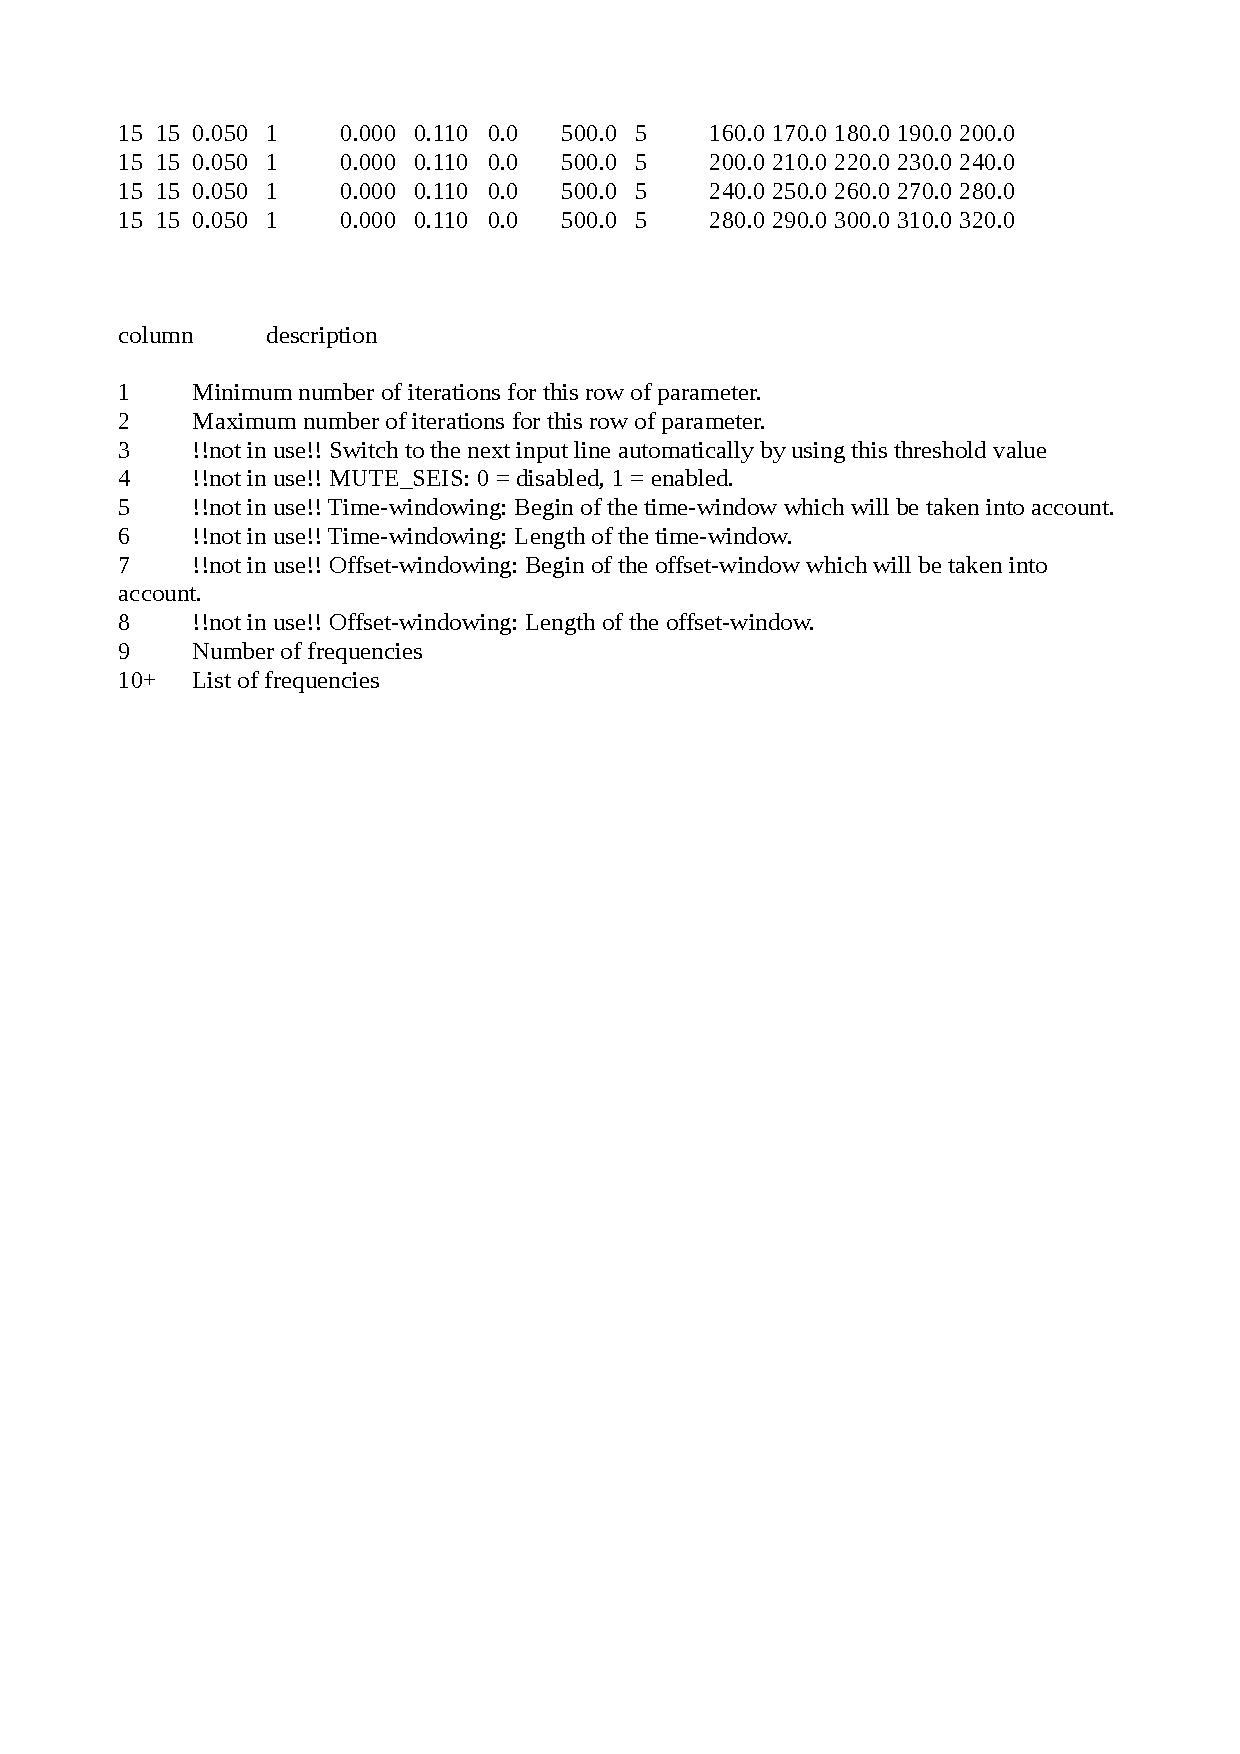
\includegraphics[width=\textwidth]{fig/workflow_input}
\caption[Workflow.dat]{The file workflow.dat organises the different inverion stages.}\label{fig:workflow_input}
\end{center}
\end{figure}
\subsection{Hessian}
\begin{verbatim}
"Hessian" : "comment",
			"HESS" : "0",
			"READ_HESS" : "0",
			"REC_HESS" : "1", 
			"WATER_HESS_VP, WATER_HESS_VS, WATER_HESS_RHO" : "0.0192, 0.0192, 1.0e-14",
			"HESS_FILE" : "./hess/toy_hess",
\end{verbatim}

If the option \textit{HESS}=1 is chosen in the input file, a diagonal Hessian approximation is applied for preconditioning of the gradients. If the Hessian approximation is already calculated it can be read from file (\textbf{READ\_HESS}=1). Hereby the hessian approximation is read from the folder \textit{hess}. The files written at the beginning of the current frequency stage are used, labeled for example \textit{hess/toy\_hess.vp\_200.00Hz\_it11} when the new frequency stage started with iteration 11. \\
For \textbf{READ\_HESS}=0 the diagonal Hessian approximation is calculated in IFOS3D as described in section~\ref{sec:hess}.\\
Due to runtime and storage it is recommendable to use only a subset of receivers for its calculation. The option \textbf{REC\_HESS} is not fully implemented at the moment, and it is therefore necessary to change the receiver file or the distance in the receiver array to its double or its triple value. \\
The water level (\textbf{WATER\_HESS}) used for the calculation of the preconditioning matrix (equation~\ref{Hess_precon}) can be estimated from the gradient of the first iteration and the diagonal Hessian matrix. It is not calculated directly in IFOS3D. This results in the fact, that it is not possible to perform a full inversion at a stretch, but the inversion needs to be split up into the different inversion stages.\\
The diagonal Hessian matrix is stored in the folder \textit{hess} and is labeled \\e.g. \textit{hess/toy\_hess.vp\_200.00Hz\_it11}. It is calculated at the beginning of each frequency stage and is applied within this frequency stage.
\subsection{L-BFGS}
\begin{verbatim}
"L-BFGS" : "comment",
			"LBFGS" : "0",
			"NUMPAR" : "2",
			"BFGSNUM" : "5"
\end{verbatim}

If \textbf{LBFGS}=1 the L-BFGS method is applied as described in section~\ref{sec:lbfgs}. The L-BFGS approach can only be used combined with the Hessian preconditioning (\textbf{HESS}=1). So far we tested the L-BFGS approach only for the seismic velocities, not for density. The number of inverted parameter classes (\textbf{NUMPAR}) can thus be chosen as 1 ($v_p$ only) or 2 ($v_p$ and $v_s$).\\
The L-BFGS algorithm estimates the Hessian from changes in gradients and models of the previous \textbf{BFGSNUM} iterations. 

\section{IFOS3D output}
\subsection{ifos3D.out}
The proceedings of the inversion can be followed in the file \textit{in\_and\_out/ifos3D.out} written by the first processor (MYID=0). This file gives information about parameters used in IFOS3D, grid dispersion and stability of the code. The proceedings of the forward modelings and output of the different sub-programs can be viewed. In case of an early termination of the program this file can be checked for an error message.
\subsection{ifos3D\_invers.out}
The output of misfit values and steplength information is written to \textit{in\_and\_out/ifos3D\_invers.out} during the run. The following values given for each iteration show the proceedings of the inversion:
\begin{itemize}
\item parameters as defined in the current iteration: the parameter \textbf{cdf} (set to one for the first iteration in each inversion stage), the lowest frequency used in this iteration and the number of frequencies for this stage. 
 \item misfit value (time domain) for each shot (\textbf{L2}), summed over shots (\textbf{L2all}) and misfit used for steplength calculation (\textbf{misfit[0]})
 \item test steplengths used for steplength estimation (\textbf{steplength}) and the resulting L2 misfits
 \item the steplength parabel and possible warnings given by \textit{src/steplength.c}
 \item the ''optimal`` steplength used for the model update and the estimated misfit for this steplength
 \item the new test steplength
\end{itemize}
If problems in the inversion occure this becomes generally quickly visible in its converge and in problems to find an optimum steplength.


\clearpage
\chapter{Toy example - the box model}
This chapter describes the inversion of a simple toy example with IFOS3D, which is a subdivided box in a homogeneous full space. This example can be performed as a first synthetic application to test IFOS3D on your system. The necessary input files and scripts are included in the IFOS3D folders and you can follow the following guidelines to perform a successfull inversion.  Your results can be compared to those given in this chapter.\\
The 3D inversion is costly even for a simple model. To enable a successfull inversion we therefore recommend the use of a  parallel system with a larger number of CPU's as for example found in supercomputing centers. We performed this inversion using 512 CPU's for 7.5 hours. Before starting this toy example, IFOS3D needs to be installed on your system (see chapter~\ref{Gettingstarted}).
\section{Inversion setup}
\subsection{Model and grid system}
\begin{figure}[h!]
\begin{center}
\includegraphics[width=\textwidth]{fig_toy/toy_real_model_neu}
\caption[Toy example - the real model and acquisition geometry]{The toy example - real model $v_p$ (a) and $v_s$ (b), sources and receivers indicated as stars and crosses, respectively}\label{fig:toy_model}
\end{center}
\end{figure}
The true model for the seismic velocities is plotted in figure~\ref{fig:toy_model}. A box divided into four differently-sized parts with different positive and negative velocity variations is placed into a homogeneous full space of $v_p=6200$\,m/s and $v_s=3600$\,m/s. The $v_p$/$v_s$ ratio is not constant.
The density model is homogeneous with 2800\,kg/m$^3$ and kept constant during inversion. The elastic model is generated in IFOS3D on the fly (\textbf{READMOD}=0) using the function \textit{src/hh\_toy.c} as defined in \textit{src/Makefile}.\\
The model size is 128\,m$\times$128\,m $\times$147.2\,m in $x$-, $z$- and $y$-direction. We use a grid point distance of \textbf{DX}=\textbf{DZ}=\textbf{DY}=0.8\,m and thus a grid size of \textbf{NX}=160, \textbf{NZ}=160 and \textbf{NY}=184 points. \\
We use spatial FD-operators of \textbf{FDORDER}=4 and Holberg coefficients (\textbf{FDCOEFF=2}). This fullfills the dispersion criterion (see SOFI manual) up to a frequency of 500\,Hz ($v_{s,min}=3450$\,m/s):
\begin{equation}
 dh <= \frac{v_{s,min}}{nf_{max}}=\frac{v_{s,min}}{8.32f_{max}}
\end{equation}
For our maximum frequency of 320\,Hz used for inversion this is well sufficient. \\
The total calculation time is \textbf{TIME}=0.06\,s with a time stepping of 5e$^{-5}$s resulting in 1200 tiesteps per forward modeling. The stability criterion is fullfilled ($v_{p,max}=6700$\,m/s):
\begin{equation}
 dt<=\frac{dh}{0.487v_{p,max}}=2.4e^{-4}
\end{equation}
The model does not contain a free surface (\textbf{FREE\_SURF}=0) and as boundary condition we use a PML-layer (\textbf{FW}) of 10 grid points width at each model side.\\
\subsection{Sources and receivers}
\begin{figure}[h!]
\begin{center}
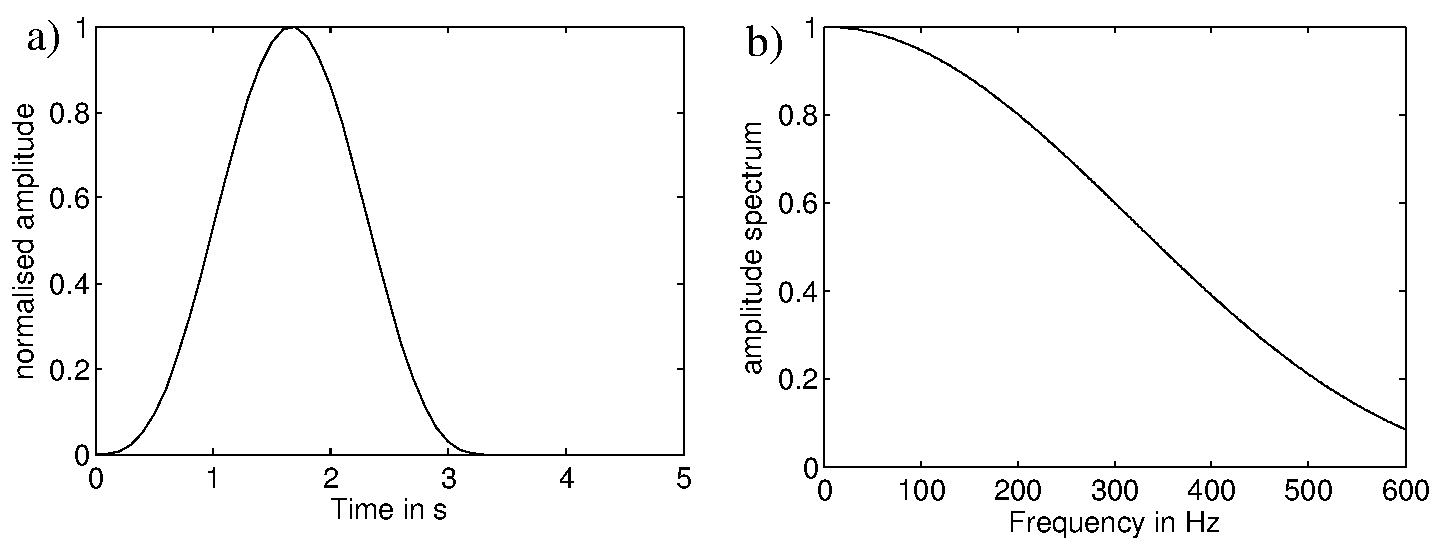
\includegraphics[width=0.8\textwidth]{fig_toy/source_toy}
\caption[Toy example - source wavelet and spectrum]{The toy example - normalised amplitude and spectrum of sin$^3$-source wavelet }\label{fig:toy_wavelet}
\end{center}
\end{figure}
Sources and receivers are arranged within $x$-$z$-planes, as indicated in Figure~\ref{fig:toy_model}. The sources are listed in \textit{sources/sources\_toy.dat} (\textbf{SOURCE\_FILE}). We use 12 (3$\times$4) sources in 92\,m depth with a central frequency of \textbf{FC}=300\,Hz. The sources are vertical directed point forces (\textbf{QUELLTYP}=4) with sin$^3$-wavelets (\textbf{QUELLART=4}) as source time functions. The corresponding source wavelet can be seen in figure~\ref{fig:toy_wavelet}a. This source wavelet comprises the low frequencies with $40\%$ of the maximum amplitude left at about 400\,Hz (figure~\ref{fig:toy_wavelet}b). \\
The receivers are arranged using a horizontal receiver array (\textbf{READREC}=2, \textbf{REC\_ARRAY}=1) in 24\,m depth. The distance between the receivers is \textbf{DRX}=\textbf{DRZ}=10 gridpoints, which gives a total number of 169 receivers. 
\subsection{Inversion parameters}
For the inversion we use homogeneous starting models with $v_s=3600$\,m/s and $v_p=6200$\,m/s. In total 60 iterations are performed (\textbf{ITMIN, ITMAX }= 1, 60) and five frequencies are employed simultanously (\textbf{NFMAX}=5). For preconditioning of gradients a local taper is applied around source and receiver positions (\textbf{DAMPTYPE}=2). We do not use the diagonal Hessian approximation (\textbf{HESS}=0) or the L-BFGS method (\textbf{LBFGS}=0). Out of the total number of 12 shots we use 4 shots for the steplength estimation (\textbf{NSHOTS\_STEP}=4) and start with an initial test steplength of 0.02 (\textbf{TESTSTEP}=0.02). The filenames for gradient and model output are given in the input file.
\subsubsection*{The workflow}
The workflow file \textit{in\_and\_out} defines the different frequency stages. They are listed in table~\ref{tab:toy_fstage}.\\
\begin{table}[h!]
\centering 
\begin{tabular}{|c|c|c|c|}\hline
 iteration& frequencies in Hz & $\lambda_{min}(v_p)$ in m &$\lambda_{min}(v_s)$ in m \\
 1-15& 160,170,180,190,200 & 31 & 18\\
16-30& 200,210,220,230,240 & 26 & 15\\
31-45& 240,250,260,270,280 & 22 & 13\\
46-60& 280,290,300,310,320 & 19 & 11\\
\hline
\end{tabular}
\caption[Transmission example: frequency stages]{Frequency stages used for the transmission geometry box example with minimum wavelengths $\lambda_{min}(v_p)$ and $\lambda_{min}(v_s)$.}
\label{tab:toy_fstage}
\end{table}
We used four frequency stages with five frequencies, which increase from stage to stage. The frequency bands are slightly overlapping. The table also lists the minimum and maximum wavelengths, which define the resolution of the result. In the first stage lower frequencies enable the reconstruction of rough model structures, whereas higher frequencies and smaller wavelengths result in a higher resolution of smaller model structures.
\section{Step by step guideline}
\subsection{Step 1 - forward modeling}
In a first step, a forward modeling is performed to calculate data of the box model, which can be used as observed data in the inversion. This corresponds to a SOFI3D simulation. The model is created on the fly by the function \textit{src/hh\_toy.c}. The parameters are already set in \textit{in\_and\_out/ifos3D\_toy.inp}. For the forward modeling we use \textbf{METHOD}=0. The seismograms are written in the folder \textit{su\_obs}. For the option \textbf{METHOD}=0 the seismograms are written in one file for each processor containing receiver locations. From these files the data can be directly used as input in the inversion. Note, that \textbf{FILT}=0 and the program calculates the unfiltered seismograms. The box model is saved in the folder \textit{model}.\\
To perform the modeling the following steps are applied:
\begin{itemize}
 \item compile IFOS3D (execute \textit{./compileIFOS3D.sh})
 \item adapt processor number in \textit{in\_and\_out/ifos3D\_toy.inp} and your job script (e.g. \textit{startIFOS3D.sh})
 \item start IFOS3D (e.g. execute \textit{./startIFOS3D.sh})
\end{itemize}
The progress of IFOS3D can be viewed in \textit{in\_and\_out/ifos3D\_toy.out}. 
\subsection{Step 2 - the FWI}
In a second step, the inversion is performed. Before starting the inversion perform the following steps:
\begin{itemize}
 \item set the parameter (kasten=0) in \textit{src/hh\_toy.c} to gain homogeneous starting models
 \item compile IFOS3D (execute \textit{./compileIFOS3D.sh})
 \item change the following parameters in \textit{in\_and\_out/ifos3D\_toy.inp}: \textbf{METHOD}=1, \textbf{FILT}=1, \textbf{SEIS\_FILE} = ./su/cal\_toy
 \item start IFOS3D (e.g. execute \textit{./startIFOS3D.sh})
\end{itemize}
Now the inversion is performed. The proceedings of IFOS3D can be seen in the outputfile \textit{in\_and\_out/ifos3D.out}. An overview how the inversion succeeds, e.g. misfit values and steplengths can be found in the output file \textit{in\_and\_out/ifos3D\_invers.out}. Both files are written during simulation.
\section{Results}
In this section we look at the output of IFOS3D and show the inversion results. All output is located in the folder \textit{par}. For processing and plotting of data we use Matlab programs, located in the folder \textit{mfiles} and Seismic Unix.
\subsection{Seismograms}
\subsubsection*{Output}
The observed seismograms are calculated in step 1- forward modeling. They are located in the folder \textit{su\_obs} and provide unfiltered particle velocities for each shot and component in the su-format (e.g. \textit{obs\_toy\_vx\_it1.su.shot3}). \\
The inverted seismograms are stored in each iteration for each shot and each component in the folder \textit{su}. They are also in the su-format and named for instance \textit{cal\_toy\_vy\_it30.su.shot2}. Note that these data are filtered below the highest frequency used within the corresponding frequency stage.\\
The su-header in front of each trace contains i.a. information about source and receiver location, time stepping and time samples. It can be viewed using the Seismic Unix function \textit{surange} $<$ FILENAME or the Matlab function \textit{su2matlab}. 
\subsubsection*{Data plot}
For a first look, the seismograms can be plotted with the SU-routine \textit{suxwigb} $<$ FILENAME. Note, that it can be necessary to use the function \textit{segyclean} $<$ FILENAME $>$ FILENAME\_OUT before plotting.\\
For a comparison of observed and inverted data, it is necessary to apply a lowpass filter to the observed data, using the maximum frequency of the corresponding stage. Figure~\ref{fig:toy_seismo1} shows a comparison between initial, observed and inverted seismograms for one source and receiver and $x$-, $z$- and $y$-component of the particle velocity. Note, that the observed data was filtered with the maximum frequency of the first iteration for a comparison in a) and with the maximum inversion frequency for a comparison with the final inverted data in b). The plot was produced with the Matlab program \textit{seismo\_trace\_toy.m}. This program uses the binary format as input, which is why the files need to be transformed before use, applying the SU-routine \textit{sustrip} $<$ FILENAME $>$ FILENAME\_OUT.
\begin{figure}[h!]
\begin{center}
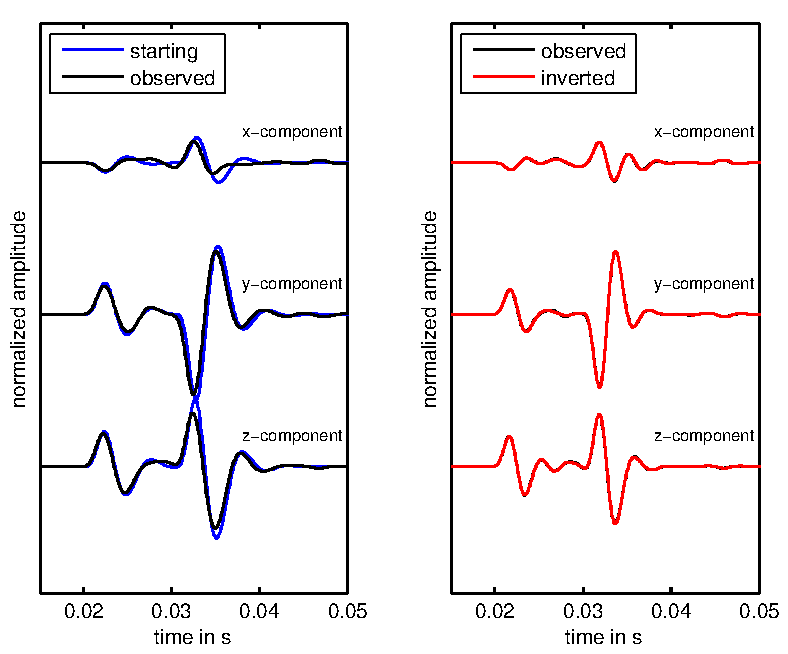
\includegraphics[width=\textwidth]{fig_toy/seismo_trace_toy}
\caption[Toy example - observed, initial and inverted seismograms]{Multi-component seismograms exemplarily for source at ($x_s$, $z_s$, $y_s$) = (32\,m, 96\,m, 92\,m) and receiver at ($x_r$, $z_r$, $y_r$) = (56\,m, 40\,m, 24\,m), normalised to one trace a) initial vs. observed data filtered below 200\,Hz and b) observed vs. inverted data filtered below 320\,Hz} \label{fig:toy_seismo1}
\end{center}
\end{figure}
\subsubsection*{Discussion}
Figure~\ref{fig:toy_seismo1} shows the comparison of initial and observed data for the low frequencies of the first inversion stage. The waveforms show only small differences and clearly no cycle skipping. Thus the homogeneous starting model is already sufficient for this simple example. \\
The success of the inversion can be seen when comparing the observed and inverted data. The waveforms, including the small oscillations are fitted very well for all components.
\subsection{The gradient} 
Gradients for $v_p$, $v_s$ and $\rho$ are stored in binary format in each iteration in the folder \textit{grad} (e.g. \textit{toy\_grad.vp\_200.00Hz\_it5}). Additionally to the raw gradients named by iteration number, the conjugate gradients are stored with labels of (iteration number +2000), like  (e.g. \\ \textit{toy\_grad.vp\_200.00Hz\_it2005}). \\
The gradients can be plotted with the Matlab program \textit{slice\_3D\_toy\_grad.m}. This program plots the 3D grid as two perpendicular slices. The acquisition geometry of the toy example is also included. \\
Here, we show the ``raw'' gradients and the preconditioned gradients of $v_p$ and $v_s$ normalised to their maximum value for the first iteration (figure~\ref{fig:toy_grad}). In the raw gradients (a,b) the high amplitudes around sources and receivers are clearly visible. Especially the source artefacts are very distinct compared to the small scaled receiver artefacts. By preconditioning these artefacts can be removed for the greater part (c,d) and the main update concentrates on the box area. Due to the smaller wavelengths of the shear wave, the $v_s$-gradient already shows more structure than the $v_p$-gradient. 
\begin{figure}[h!]
\begin{center}
\includegraphics[width=\textwidth]{fig_toy/grad_toy_neu}
\caption[Toy example - gradient before and after preconditioning]{Normalised gradients of first iteration : a) ``raw'' gradient $v_p$, b) ``raw'' gradient $v_s$, c) preconditioned gradient $v_p$ and d) preconditioned gradient $v_s$; sources (stars) and receivers (crosses) are indicated. }\label{fig:toy_grad}
\end{center}
\end{figure}
\subsection{Misfit and steplength proceedings}
The misfit and steplength values are stored in \textit{in\_and\_out/ifos3D\_invers.out}. They give insights into the proceedings of the inversion. After storing the values one in a row in textfiles, they can be plotted with the Matlab functions \textit{misfit\_toy.c} and \textit{steplength\_toy.c}. \\
The misfit proceedings are plotted in figure~\ref{fig:toy_misfit}. The values are normalised to the initial misfit. The curve shows a high convergence at the beginning of the inversion, where the rough model structures are included. The curve flattens as the inversion proceeds and only finer changes in the model are performed. Note, that with each new frequency stage data is added to the misfit and the misfit steps to higher values, which is then reduced within this stage.\\
\begin{figure}[h!]
\begin{center} 
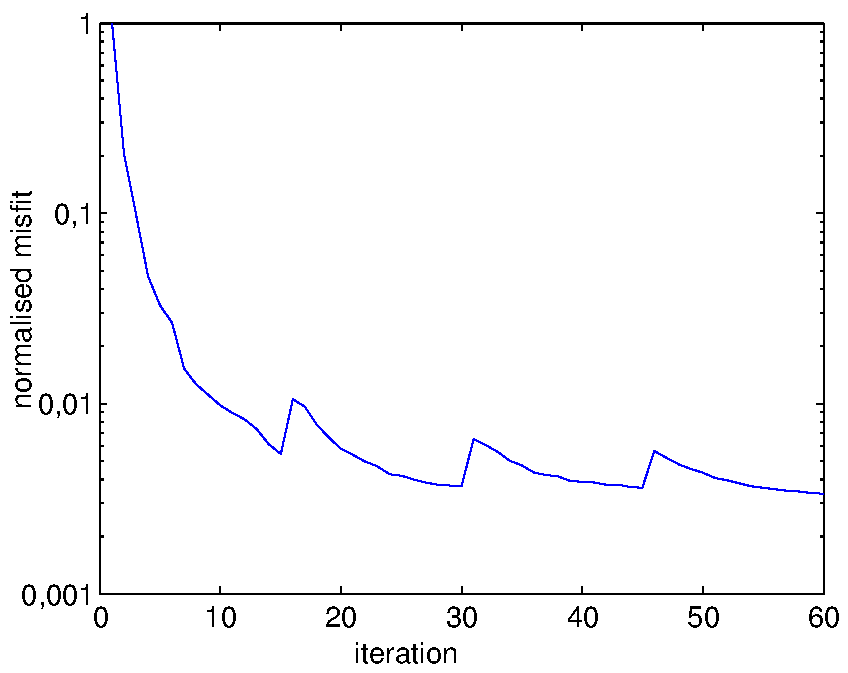
\includegraphics[width=0.7\textwidth]{fig_toy/toy_misfit}
\caption[Toy example - misfit]{Misfit normalised to initial value shows the convergence }\label{fig:toy_misfit}
\end{center}
\end{figure}
The steplength curve (figure~\ref{fig:toy_steplength}) shows a similar behaviour. At the beginning steplengths of few percent are found. That means the size of the model update is few percent of the average model parameter. These steplengths quickly decrease to less than 0.5\% after few iterations. Most model changes are thus made in the first few iterations whereas only the fine work is performed in the later iterations and at higher frequencies.
\begin{figure}[h!]
\begin{center}
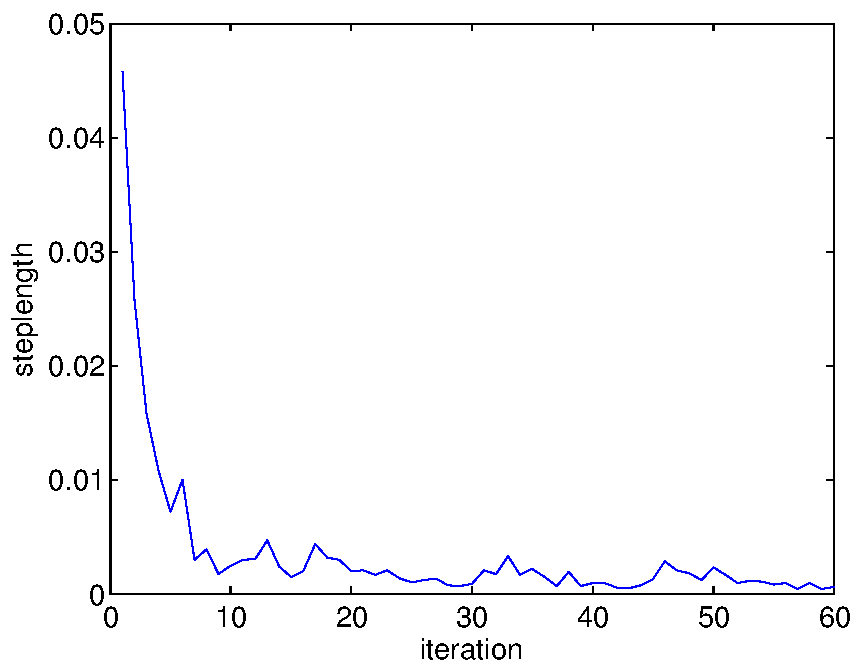
\includegraphics[width=0.7\textwidth]{fig_toy/toy_steplength}
\caption[Toy example - misfit]{Steplength proceedings}\label{fig:toy_steplength}
\end{center}
\end{figure}

\subsection{The final models}
Model parameters are written into the folder \textit{model} in each iteration for each parameter ($v_p$, $v_s$, $\rho$) in binary format (e.g. \textit{toy.vp\_it22}). They can be plotted similarly to the gradient with the program \textit{slice\_3D\_toy\_model.m}. Note, that gradient and model files share the same structure.\\
The results for the toy example is plotted for two 2D slices. Figure~\ref{fig:toy_result1} shows a horizontal slice through the box area. The three different box areas seen in the real model in a) and c) are well resolved for $v_p$ (b) and $v_s$ (d) after 60 iterations. However the $v_s$-model offers a clearly higher resolution due to the smaller wavelengths compared to the $v_p$-model. In transmission geometry a resolution down to one wavelength is possible and higher frequencies would be necessary to gain a better resolved box in $v_p$.
\begin{figure}[h!]
\begin{center}
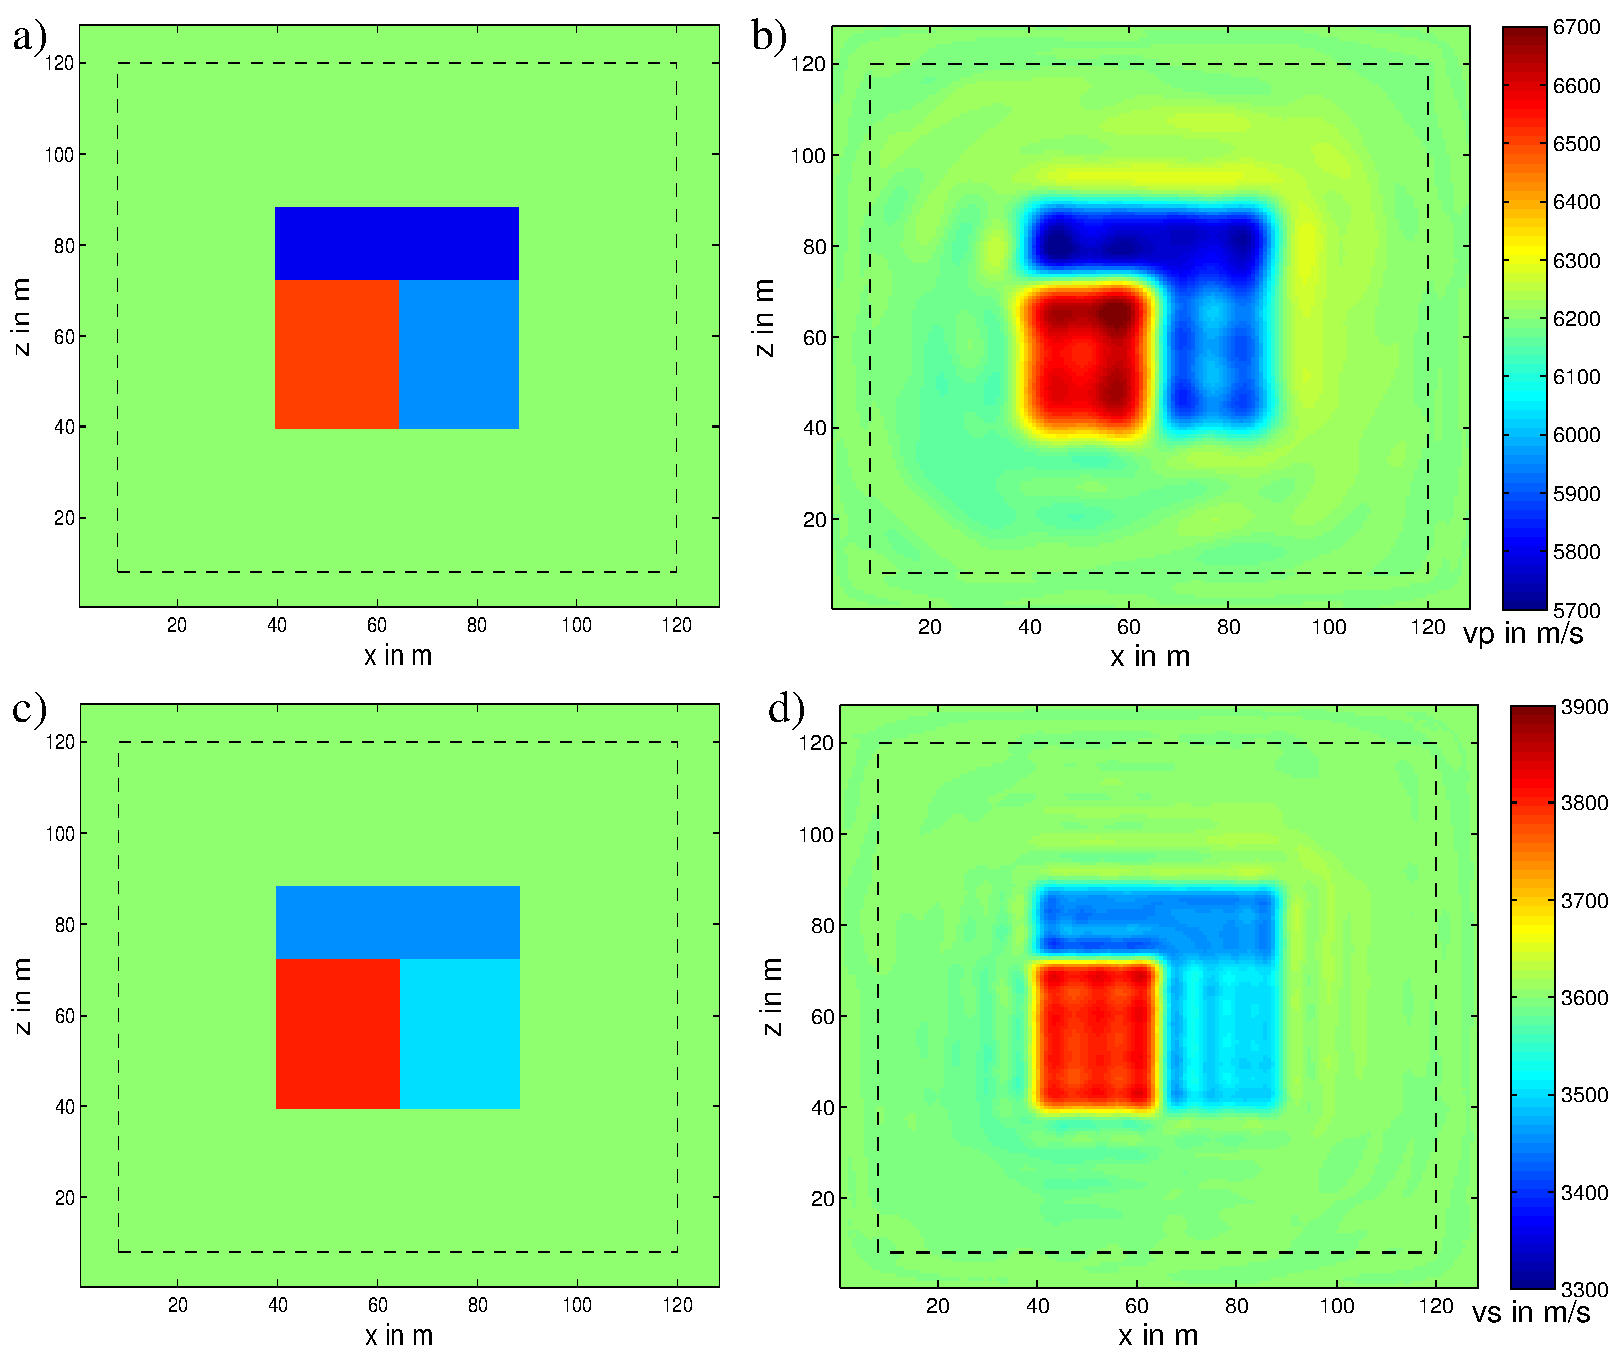
\includegraphics[width=\textwidth]{fig_toy/toy_model_result_new}
\caption[Toy example - final inverted models, horizontal slice]{Final inverted models (60 iterations) compared to real models for horizontal slice at $y$=60\,m: a) real model $v_p$, b) inverted  model $v_p$, c) real model $v_s$ and d) inverted model $v_s$. The dashed line indicates the absorbing frame;  }\label{fig:toy_result1}
\end{center}
\end{figure}
A vertical slice of the models is plotted in figure~\ref{fig:toy_result2}. Overall, the vertical direction is more difficult to reconstruct, as can be ssen in the inverted models of $v_p$ (b) and $v_s$ (d) compared to the real models (a,b). The boundaries of the box are relatively well recovered for both parameters. The inversion of $v_p$ reconstructs the two main areas of the box, however the small high velocity area (dark red) cannot be resolved. This area is indicated in the inverted $v_s$ model, again showing the higher resolution of this parameter.
\begin{figure}[h!]
\begin{center}
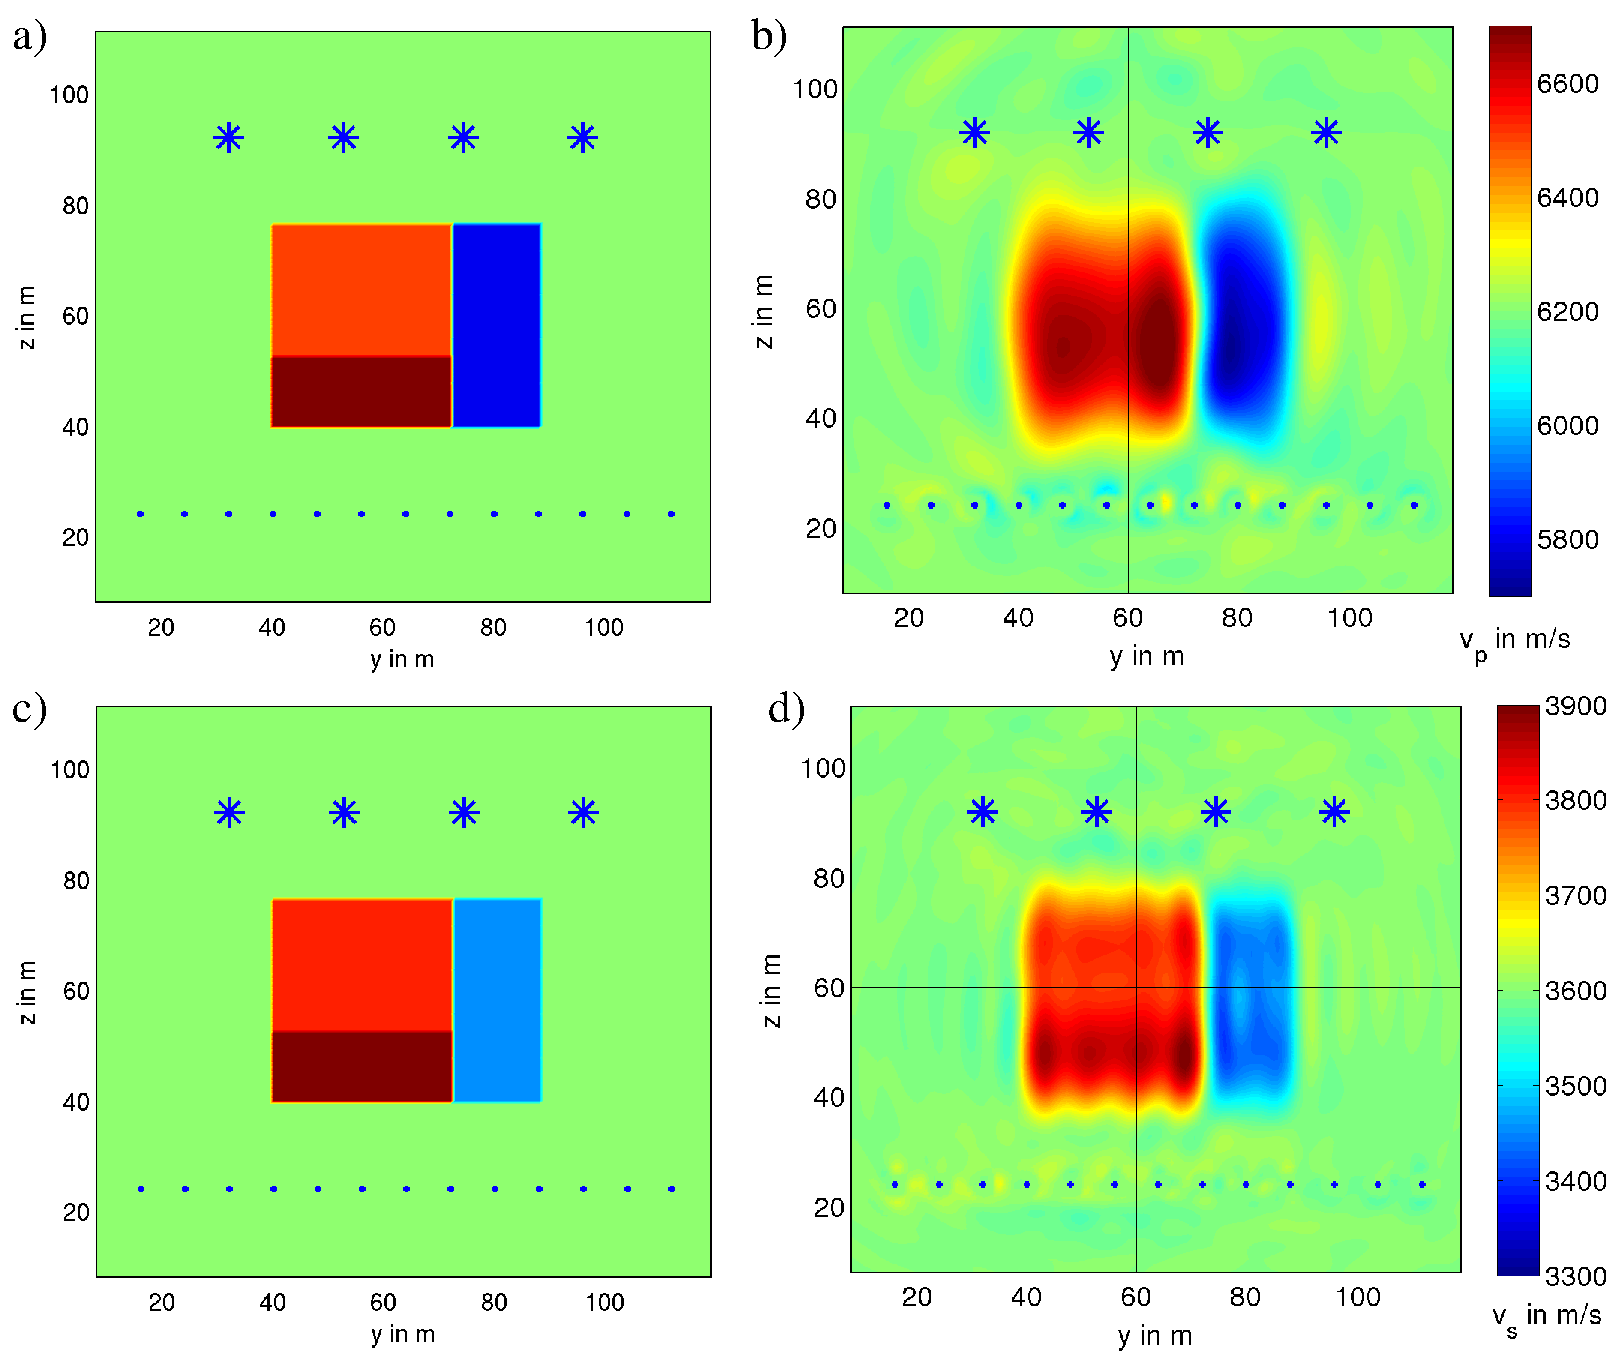
\includegraphics[width=\textwidth]{fig_toy/toy_model_result1}
\caption[Toy example - final inverted models, vertical slice]{Final inverted models (60 iterations) compared to real models for vertical slice at $x$=56\,m: a) real model $v_p$, b) inverted  model $v_p$, c) real model $v_s$ and d) inverted model $v_s$; }\label{fig:toy_result2}
\end{center}
\end{figure}

\section{Outlook}
This example is also included by \cite{But15}. Here the applications using the diagonal Hessian approximation and the L-BFGS method are shown. You can also look at the other applications \citep{But13, But15} which include the inversion of a random medium model in different transmission geonetries and a surface geometry model.



\clearpage

\phantomsection
\addcontentsline{toc}{chapter}{Bibliography}
\bibliographystyle{gji}
\bibliography{manual_IFOS3D}


\begin{appendix}
\chapter{Source code short description}\label{sec:code_overview}
In the following we will give a short overview about the different programs of the IFOS3D source code.\\
\\
\textbf{ifos3d} - main program.\\
\\
\textbf{Makefile} - makefile for IFOS3D.\\
\\
\textbf{fd.h} - include file for IFOS3D. \\
\\
\textbf{globvar.h} - defines global variables for IFOS3D.\\

\subsection*{Subprograms}
\textbf{absorb.c} - calculation of absorbing boundary coefficients using exponential damping \citep{Cer85}.\\
\\
\textbf{av\_mat.c} - averaging material parameters for the staggered-grid\\
\\
\textbf{checkfd\_ssg.c} - check for stability, grid dispersion and the accessibility of data output directories and files. \\
\\
\textbf{comm\_ini.c} - initialisation of repeated comunications. This may reduce the network overhead.\\
\\
\textbf{conjugategrad.c} - calculation of the conjugate gradient direction (MORA, 1987).\\
\\
\textbf{CPML\_coeff.c} - defining damping profiles for CPML boundary condition. This C-PML implementation is adapted from the 2nd order isotropic CPML code
 by Dimitri Komatitsch and based in part on formulas given in Roden and Gedney (2000). \\
\\
\textbf{CPML\_ini\_elastic.c} - definition of CPML boundary domains for each submodel.\\
\\
\textbf{cpmodel.c} - copying of model parameters into a testmodel.\\
\\
\textbf{disc\_fourier.c} - calculation of a discrete Fourier transfomation on the fly: Fouriercomponents of forward or backpropagated wavefields are summed up for each frequency.\\
\\
\textbf{exchange\_Fv.c} - exchange of wavefield velocities (frequency donain) at grid boundaries between processors.\\
\\
\textbf{exchange\_par.c} - exchange of input parameters between processors.\\
\\
\textbf{exchange\_s.c} - exchange of stress values at grid boundaries between processors.\\
\\
\textbf{filt\_seis.c} - filtering of seismograms in time domain with a Butterworth filter of the libseife library. Lowpass or highpass filtering can be applied.  \\
\\
\textbf{gradient\_F.c} - gradient calculation in frequency domain: gradient as multiplication of forward and conjugate backpropagated wavefield spatial derivatives are calculated by 4th order finite differences.\\
\\
\textbf{hess\_apply.c} - preconditioning of gradient with diagonal Hessian approximation.\\
\\
\textbf{hess\_F.c} - calculation of diagonal Hessian approximation in frequency domain.\\
\\
\textbf{hh.c} - generation of an elastic or viscoelastic model specified by $v_p$, $v_s$ and $\rho$.\\
\\
\textbf{info.c} - printing information about IFOS3D.\\
\\
\textbf{initproc.c} - dividing the 3-D FD grid into domains and assigning the processors to these domains,\\
\\
\textbf{lbfgs.c} - calculation of L-BFGS update.\\
\\
\textbf{lbfgs\_save.c} - saving gradient for L-BFGS calculation; only first iteration, later saved in lbfgs.c.\\
\\
\textbf{matcopy.c} - exchange of model parameters to neighbouring processors for the averaging of material properties.\\
\\
\textbf{merge.c} - merge snapshots files written by the different processes to a single file. \\
\\
\textbf{mergemod.c} - merge model files written by the different processes to a single file. Used for gradients and model output in IFOS3D. \\
\\
\textbf{model2\_5D.c} - creation of a 2.5D model from a 3D model, (attention: not in parallel!!); 2.5D model parameters constant in z-direction.\\
\\
\textbf{modelupdate.c} - update of model for next iteration.\\
\\
\textbf{note.c} - writing note to stdout.\\
\\
\textbf{outgrad.c} - output of gradients to GRAD\_FILE.\\
\\
\textbf{outmod.c} - output of model parameters $v_p$, $v_s$ and $\rho$ to MOD\_OUT\_FILE.\\
\\
\textbf{output\_source\_signal.c} - output source signal e.g. for cross-correlation, deconvolution or comparison with analytical solutions. \\
\\
\textbf{outseis.c} - writing seismograms to disk. \\
\\
\textbf{precongrad.c} - gradient preconditioning around sources, receivers and at model boundaries.\\
\\
\textbf{psource.c} - generation of explosive source at source nodes.\\
\\
\textbf{rd\_sour.c} - reading external source wavelet.\\
\\
\textbf{read\_checkpoint.c} - reading wavefield from checkpoint file.\\
\\
\textbf{readdsk.c} - reading one single amplitude from file.\\
\\
\textbf{readhess.c} - reading Hessian from files.\\
\\
\textbf{readinv.c} - reading inversion parameters from workflow.\\
\\
\textbf{readmod.c} - reading elastic model properties ($v_p$, $v_s$, density) from file.\\
\\
\textbf{read\_par.c} - reading FD-Parameters from input-file. \\
\\
\textbf{readseis.c} - reading seismograms from files.\\
\\
\textbf{receiver.c}  - finding global grid positions for the receivers.\\
\\
\textbf{residual.c} - calculation of data residuals (displacement) and L2 norm.\\
\\
\textbf{rwsegy.c} - reading and writing SEG-Y, SU, BIN, TXT and UKOOA P190.\\
\\
\textbf{save\_checkpoint.c} - saving wavefield to checkpoint file.\\
\\
\textbf{saveseis.c} - writing seismograms to files.\\
\\
\textbf{segy.h} - include file for SEGY traces.\\
\\
\textbf{seismerge.c} - merging SEG-Y files.\\
\\
\textbf{seismo\_ssg.c} - storing amplitudes (particle velocities or pressure) at receiver positions in arrays.\\
\\
\textbf{smooth.c} - smoothing model parameters (complete model or boundaries only), not in parallel.\\
\\
\textbf{snapmerge.c} - loop over snapshotfiles which have to be merged.\\
\\
\textbf{snap\_ssg.c} - writing 3D snapshot for current timestep to disk.\\
\\
\textbf{sources.c} - reading source parameters from  source file.\\
\\
\textbf{splitrec.c} - computation of local receiver coordinates (within each subgrid). \\
\\
\textbf{splitsrc.c} - computation of local source coordinates (within each subgrid).\\
\\
\textbf{steplength.c} - steplength calculation using a parabola method.\\
\\
\textbf{surface\_ssg.c} - stress free surface condition using the mirroring technique.\\
\\
\textbf{surface\_ssg\_elastic.c} - stress free surface condition, elastic case.\\
\\
\textbf{timing.c} - output timing information (real time for updates etc.).\\
\\
\textbf{update\_s\_ssg.c} - updating stress values by a staggered grid finite difference scheme of nth order accuracy in space and second order accuracy in time (viscoelastic version).\\
\\
\textbf{update\_s\_ssg\_CPML.c} - updating stress values in the CPML-boundaries (4th order spatial FD sheme) (viscoelastic version).\\
\\
\textbf{update\_s\_ssg\_CPML\_elastic.c} - updating stress values in the CPML-boundaries (4th order spatial FD sheme) (elastic version).\\
\\
\textbf{update\_s\_ssg\_elastic.c} - updating stress values by a staggered grid finite difference scheme of nth order accuracy in space and second order accuracy in time (elastic version).\\
\\
\textbf{update\_v\_ssg.c} - updating velocity values by a staggered grid finite difference scheme of nth order accuracy in space and second order accuracy in time.\\
\\
\textbf{update\_v\_ssg\_CPML.c} - updating velocity values in the CPML-boundaries (4th order spatial FD sheme).\\
\\
\textbf{util.c} - some utility-routines from numerical recipes \citep{pre90}.\\
\\
\textbf{wavelet.c} - Calculating source signal at different source positions for input source parameters.\\
\\
\textbf{writedsk.c} - writing one single amplitude on disk.\\
\\
\textbf{writemod.c} - writing local model to file (not in use, see outmod).\\
\\
\textbf{writepar.c} - writing FD-Parameter to output file stdout or log-file.\\
\\
\textbf{zero\_grad.c} - initialise gradient with zero.\\
\\
\textbf{zero\_invers.c} - initialise wavefield (frequency domain) with zero.\\
\\
\textbf{zero\_wavefield.c} - initialise wavefield with zero.\\
\end{appendix}

%\cleardoublepage
%\input{Danksagung.tex} 

\end{document}
